 %%%%%%%%%%%%%%%%%%%%%%% file template.tex %%%%%%%%%%%%%%%%%%%%%%%%%
 %
 % This is a general template file for the LaTeX package SVJour3
 % for Springer journals.          Springer Heidelberg 2010/09/16
 %
 % Copy it to a new file with a new name and use it as the basis
 % for your article. Delete % signs as needed.
 %
 % This template includes a few options for different layouts and
 % content for various journals. Please consult a previous issue of
 % your journal as needed.
 %
 %%%%%%%%%%%%%%%%%%%%%%%%%%%%%%%%%%%%%%%%%%%%%%%%%%%%%%%%%%%%%%%%%%%
 %
 % First comes an example EPS file -- just ignore it and
 % proceed on the \documentclass line
 %% your LaTeX will extract the file if required
 %\begin{filecontents*}{example.eps}
 %%!PS-Adobe-3.0 EPSF-3.0
 %%%BoundingBox: 19 19 221 221
 %%%CreationDate: Mon Sep 29 1997
 %%%Creator: programmed by hand (JK)
 %%%EndComments
 %
 %\end{filecontents*}
 %
 \RequirePackage{fix-cm}
 %
 %\documentclass{svjour3}                     % onecolumn (standard format)
 %\documentclass[smallcondensed]{svjour3}     % onecolumn (ditto)
 \documentclass[smallextended]{svjour3}       % onecolumn (second format)
 %\documentclass[twocolumn]{svjour3}          % twocolumn
 %
 \smartqed  % flush right qed marks, e.g. at end of proof
 %
 % ------------- Packages Used --------------------------------------------------
% They help us to produce a better looking document ;-)
% ------------------------------------------------------------------------------

% Comment the following line before compiling the final version
%\synctex
\usepackage{multirow}

\usepackage{graphicx}
\usepackage{alltt}
\usepackage{relsize}
%\usepackage{xspace}
\usepackage{booktabs}
\usepackage{amsmath}
%\usepackage{multirow}
%\usepackage{array}
\usepackage{verbatim}
\usepackage[table]{xcolor}
\usepackage{caption}
\usepackage[labelformat=simple, labelsep=colon]{subcaption}{}
\captionsetup{compatibility=false}

%\usepackage[tight,footnotesize]{subfigure}

%\usepackage{capt-of}
%\usepackage{pifont}
\usepackage{amsfonts}
\usepackage{amssymb}
%\usepackage[latin1]{inputenc}
%\usepackage{times}
%\usepackage{colortbl}
%\usepackage{boxedminipage}
\usepackage{float}
%\usepackage{cite}
%\usepackage{fancyvrb}
%\usepackage{hyperref}
%\usepackage{balance}
\usepackage{url}
\usepackage{fancybox}%for \hypobox
\usepackage{listings}
\usepackage{array}
\usepackage{graphicx}
\usepackage{float}
%\usepackage{placeins}
\usepackage{multirow}
%\usepackage{blindtext}
%\usepackage{lipsum}
\usepackage{graphicx}
\usepackage{float}
%\usepackage{placeins}
\usepackage{multirow}
%\usepackage{caption} 

	
%\usepackage{subcaption}
%\usepackage{blindtext}
%\usepackage{lipsum}
\usepackage{graphicx}
\usepackage{amsmath}
\usepackage{booktabs}
\usepackage{framed}
\usepackage{multirow}% http://ctan.org/pkg/multirow
\usepackage{hhline}% http://ctan.org/pkg/hhline
\usepackage{amssymb}% http://ctan.org/pkg/amssymb
\usepackage{pifont}% http://ctan.org/pkg/pifont
\newcommand{\cmark}{\ding{51}}%
\newcommand{\xmark}{\ding{55}}%
%\usepackage{makecell}
%\usepackage{tablefootnote}

%\usepackage{textcomp}
%\usepackage{latexsym}
%\usepackage{amssymb}
%\usepackage{stmaryrd}
%\usepackage{euscript}
%\usepackage{wasysym}
%\usepackage{pifont}
%\usepackage{manfnt}
%\usepackage{undertilde}
%\usepackage{ifsym}
%\usepackage{tipa}
%\usepackage{txfonts}
%\usepackage{skak}
%\usepackage{skull}
%\usepackage{eurosym}
%\usepackage{yfonts}
%\usepackage{mathdots}
%\usepackage{trsym}
%\usepackage{upgreek}
%\usepackage{chemarr}
%\usepackage{accents}
%\usepackage{nicefrac}
%\usepackage{bm}


%\usepackage{pdfsync}

%   ACM Style
%\usepackage{lcsect}
% ------------------------------------------------------------------------------






% ------------ Color Definitions -----------------------------------------------
% Whatever colors we need
% ------------------------------------------------------------------------------
\definecolor{mygray}{rgb}{0.7,0.7,0.7}
% ------------------------------------------------------------------------------






% ---------- Special commands for annotating the paper's text ------------------
\let\mymarginpar\marginparm
\marginparwidth=1cm
\marginparsep=5pt
\newcommand{\todo}[1]{\textcolor{red}{\textbf{[[#1]]}}}
\def\TODO#1{\noindent\colorbox{yellow}{\bf \textcolor{red}{TODO: #1}}}
\newcommand{\hint}[1]{\textcolor{blue}{\textbf{#1}}}
\def\fig#1{Figure~\ref{#1}}
\def\tab#1{Table~\ref{#1}}
\def\eqn#1{Equation~\ref{#1}}
\def\sec#1{Section~\ref{#1}}

\pagenumbering{arabic}
\newcommand{\reviewer}[1]{\textcolor{DeepPink1}{{\it [Reviewer says: #1]}}}
\newcommand{\mei}[1]{\textcolor{red}{{\it [Mei says: #1]}}}
\newcommand{\ian}[1]{\textcolor{blue}{{\it [Ian says: #1]}}}
\newcommand{\nic}[1]{\textcolor{WildStrawberry}{{\it [Nico says: #1]}}}
\newcommand{\ahmed}[1]{\textcolor{green}{{\it [Ahmed says: #1]}}}
\newcommand{\myfoot}[1]{\footnote{\scriptsize #1}}
\newcommand{\myurl}[1]{\myfoot{\url{#1}}}
\newcommand{\Ra}{{$\Rightarrow$}}
\newcommand{\ra}{{$\rightarrow$}}
\newcommand{\La}{{$\Leftarrow$}}
\newcommand{\la}{{$\leftarrow$}}
\newcommand{\lra}{{$\leftrightarrow$}}
\newcommand{\LRa}{{$\Leftrightarrow$}}
%\newcommand{\todo}{\bram{todo}}

\newenvironment{myindentpar}[1]%
{\begin{list}{}%
         {\setlength{\leftmargin}{#1}}%
         \item[]%
}
{\end{list}}

% \AtBeginDocument{%
%    \renewcommand{\figurename}{Figure}%
%    \newcommand{\subfigureautorefname}{\figureautorefname}%for using subfig
% %   \renewcommand{\tablename}{TABLE}%
%    \renewcommand{\tablename}{Table}%
%    \renewcommand{\subsectionautorefname}{Section}%
%    \renewcommand{\sectionautorefname}{Section}%
% }

% Hypothesis box	
% ------------------------------------------------------------------------------	
\newcommand{\hypobox}[1]{\begin{center}%	
	\noindent\thicklines\setlength{\fboxsep}{7pt}%	
	\cornersize{0}\Ovalbox{\begin{minipage}{4.1in}%	
	\vspace{-0.1cm}
	\textit{#1}
	\vspace{-0.1cm}
	\end{minipage}} \end{center}}	
% ------------------------------------------------------------------------------




% ------------------------- SYMBOLS OF SELF NAMES OFTEN USED -------------------
\newcommand{\APACHE}{{\small APACHE}\xspace}
\newcommand{\BUGZILLA}{{\small BUGZILLA}\xspace}
\newcommand{\ECLIPSE}{{\small ECLIPSE}\xspace}
\newcommand{\ASPECTJ}{{\small ASPECTJ}\xspace}
\newcommand{\JDT}{{\small JDT}\xspace}
\newcommand{\GNU}{{\small GNU}\xspace}
\newcommand{\MOZILLA}{{\small MOZILLA}\xspace}
\newcommand{\THUNDERBIRD}{{\small THUNDERBIRD}\xspace}
\newcommand{\JAVA}{{\small Java}\xspace}
\newcommand{\GNOME}{{\small GNOME}\xspace}
\newcommand{\PG}{{\small PostgreSQL}\xspace}
\newcommand{\SIM}{{\small SimScan}\xspace}

% Anything else, e.g., \NAME{MICROSOFT}
\newcommand{\NAME}[1]{{\small #1}\xspace}
% ------------------------------------------------------------------------------




% ----------------------- Computer Science lol ---------------------------------
% Variable, function, and program names
% ------------------------------------------------------------------------------
\newcommand{\smalltt}[1]{\ifmmode{\mbox{\smaller\texttt{#1}}}\else{\smaller\tt #1}\fi}
\newcommand{\code}[1]{\smalltt{#1}}
\newcommand{\var}[1]{\code{#1}}
\newcommand{\func}[1]{\code{#1}}
\newcommand{\proc}[1]{\code{#1}}
\newcommand{\prog}[1]{\code{#1}}
\newcommand{\type}[1]{\code{#1}}
\newcommand{\progpt}[1]{\code{#1}}

\newcommand{\mypar}[1]{\vspace{.1cm}\noindent \textbf{#1}}
\newcommand{\myxpar}[1]{\vspace{.1cm}\noindent \textbf{#1}\newline}
% ------------------------------------------------------------------------------





% ----------- Things to remember -----------------------------------------------
\newenvironment{mynote}%
{ \medskip
  \noindent
  \let\emph=\textbf
  \begin{boxedminipage}{\columnwidth}\em}%
{ \end{boxedminipage}}
% ------------------------------------------------------------------------------






% -------------------- Use bars ------------------------------------------------
% These macros are for advanced presentation of results by shaded bars only!
% © Tom Zimmermann, 2008
% ------------------------------------------------------------------------------
\newdimen\qdx
\newdimen\qda
\newdimen\qdb
\def\rrrr#1#2#3#4{\newdimen\qd\qd=#4 % length of bar for 1.0
\qdx=\qd\multiply\qdx by 5\divide\qdx by 4
\qda=\qd
\qdb=\qd
\multiply\qda by #1\divide\qda by #3\multiply\qdb by #2\divide\qdb by #3\advance\qdb by -\qda
    \leavevmode\hbox to \qdx{\hfil\vbox{%
    \hbox{\vrule\vbox{\hrule\hbox to 1\qd
            {\vrule depth0pt height0.7ex width \qda\color{mygray}%
 \vrule depth0pt height0.7ex width \qdb\hfill}\hrule}\vrule}
    }\hfil}}
\def\rrr#1#2#3{\rrrr{#1}{#2}{#3}{0.8cm}}
% -------------------------------------------------------------------------






% ------------ Graphics Hacks --------------------------------------------------
% Use these settings if Figures tend to get their one separate pages
% ------------------------------------------------------------------------------
% \renewcommand{\topfraction}{0.85}
% \renewcommand{\textfraction}{0.1}
% \renewcommand{\floatpagefraction}{0.75}
% ------------------------------------------------------------------------------





% ------------------ Biblio Hack -----------------------------------------------
% Use these settings if the References take too much space
% ------------------------------------------------------------------------------
\let\oldthebibliography=\thebibliography
  \let\endoldthebibliography=\endthebibliography
  \renewenvironment{thebibliography}[1]{%
%	\vspace{-0.3cm}
    \begin{oldthebibliography}{#1}%
%	\vspace{-0.2cm}
       \setlength{\parskip}{0ex}%
       \setlength{\itemsep}{0ex}%
%	\bibfont
  }%
  {%
    \end{oldthebibliography}%
  }
% ------------------------------------------------------------------------------





% -------------- Floats Redefined ----------------------------------------------
% Use these settings to change the whitespace between floats and text
% ------------------------------------------------------------------------------

% \setlength\dblfloatsep{1pt}
% \setlength\floatsep{1pt}
% \setlength\textfloatsep{5pt}
% \setlength\dbltextfloatsep{5pt}

% \renewcommand\floatpagefraction{.9}
% \renewcommand\topfraction{.9}
% \renewcommand\bottomfraction{.9}
% \renewcommand\textfraction{.1}
% \setcounter{totalnumber}{50}
% \setcounter{topnumber}{50}
% \setcounter{bottomnumber}{50}
% ------------------------------------------------------------------------------
 \usepackage{graphicx}
 %
 % \usepackage{mathptmx}      % use Times fonts if available on your TeX system
 %
 % insert here the call for the packages your document requires
 %\usepackage{latexsym}
 % etc.
 %
 % please place your own definitions here and don't use \def but
 % \newcommand{}{}
 %
 % Insert the name of "your journal" with
 % \journalname{myjournal}
 %

\begin{document}
%
% paper title
% Titles are generally capitalized except for words such as a, an, and, as,
% at, but, by, for, in, nor, of, on, or, the, to and up, which are usually
% not capitalized unless they are the first or last word of the title.
% Linebreaks \\ can be used within to get better formatting as desired.
% Do not put math or special symbols in the title.
% Do not put math or special symbols in the title.
\title{An Empirical Study On Log Changes During Bug Fixes in Platform Systems}

\author{First Author         \and
	Second Author %etc.
}

%\authorrunning{Short form of author list} % if too long for running head

\institute{Suhas. Kabinna \at
	first address \\
	Tel.: +123-45-678910\\
	Fax: +123-45-678910\\
	\email{fauthor@example.com}           %  \\
	%             \emph{Present address:} of F. Author  %  if needed
	\and
	S. Author \at
	second address
}

\date{Received: date / Accepted: date}
% The correct dates will be entered by the editor




% make the title area
\maketitle

% As a general rule, do not put math, special symbols or citations
% in the abstract
\begin{abstract}
	Logs are leveraged by software developers to record and convey important information during the execution of a system. These logs are a valuable source of information for developers to debug large software systems. Prior research has shown that logs are changed during field debugging. However, little is known about how logs are changed during bug fixes. In this paper, we perform a  case study on three large open source platform software namely \emph{Hadoop}, \emph{HBase} and \emph{Qpid}. We find that logs are added, deleted and modified statistically significantly more during bug fixes than other code changes. Furthermore, we identify four different types of modifications that developers make to logs during bug fixes, including: (1) modification to logging level, (2) modification to logging text, (3) modification to logged variable and (4) relocation of log. We find that bug fixes that contain changes to logs have larger code churn, but involve fewer developers, require less time and have less discussion during the bug fix. This suggests that given two bugs of similar complexity, the one which leverages logs and has log changes, has likelihood of being resolved faster. We build a regression model to explore the relationship between log churn metrics and the resolution time of bugs. We find that log churn metrics can complement traditional metrics, i.e., \# of developers and \# of comments, in explaining the bug resolution. In particular, we find a negative relationship between modifying logs and the resolution time of bugs. This means that bug fixes with log modifications have higher likelihood of being resolved faster.


\end{abstract}

% no keywords




% For peer review papers, you can put extra information on the cover
% page as needed:
% \ifCLASSOPTIONpeerreview
% \begin{center} \bfseries EDICS Category: 3-BBND \end{center}
% \fi
%
% For peerreview papers, this IEEEtran command inserts a page break and
% creates the second title. It will be ignored for other modes.







\section{Introduction}

Platform software provides an infrastructure for a variety of applications that run on top of it. Platform software often relies on logs to monitor the applications that run over it. Such logs are generated through simple \textsl{printf} statements or through the use of logging libraries such as `Log4j', `Slf4j', and `JCL'. Each logging statement contains a static textual part that gives information about the context,  a variable part that contains knowledge about the events, and a logging verbosity level that indicates when the log should be output. An example of a log is shown below where \emph{info} is the logging level, \emph{Connected to} is the event and the variable \emph{host} contains the information about the logged event. 

\hypobox{ \hspace{25pt} LOG.info( ``Connected to " + host);}

 In our paper we use `log' to refer to the logging statements in the source code, and use `output log' to refer to the logs generated during system execution. We use the term `bug fix' to refer to the commits made to fix a bug, and `non-bug fix' refers to commits made during improvements, tests, new features and other tasks.
 
Research has shown that logs are used by developers extensively during the development of software systems~\cite{Characterizinglogs}. Logs are leveraged for anomaly detection~\cite{XUanomalies,ConsoleLogs,Marksyer}, system monitoring~\cite{Bitperformance}, capacity planning~\cite{IanWCRE} and large-scale system testing~\cite{markTesting}. The valuable information in logs has created a new market for log maintenance platforms such as Splunk~\cite{Bitperformance}, XpoLog~\cite{Xpolog}, and Logstash~\cite{Logstash}, which assist developers in analyzing logs.

Logs are extensively used to help developers fix bugs in platform software. For example, in the JIRA issue HBASE-3403\footnote{https://issues.apache.org/jira/browse/HBASE-3403}, a bug was reported when a region is orphaned when system failure occurs during a split. Developers leveraged logs to identify the point of failure. After fixing the bug, the logs were updated to prevent similar bugs from re-occurring. A recent study shows that changes to logs have a strong relationship with code quality~\cite{EMSEIAN}. However, there exists no large scale study that investigate how logs are changed during bug fixes.  This information is necessary as previous research shows that 16-32\% of logs changes are made during field debugging~\cite{EMSEIAN}, but how these changes are made is not understood. 


In this paper, we perform an empirical study on the changes that occur to logs during bug fixes in three open source platform software, i.e., \emph{Hadoop}, \emph{HBase} and \emph{Qpid}. In particular, we sought to answer the following research questions. 

\begin{description}
\item[\textbf{RQ1:}]\textbf{Are logs changed more often during bug fixes?} 

We find that logs are changed more often during bug fixes than non-bug fixes. In particular, we find that adding and modifying logs occurs more often in bug fixes than non-bug fixes (statistically significant with non-trivial effect size). We identified four types of modifications to logs, including \emph{modification to logging level}, \emph{modification to logging text}, \emph{modification of logged variable} and \emph{relocation of log}. We find that \emph{modification to logging text}, \emph{modification of logged variable} and \emph{relocation of log} occur more often in bug fixes than non-bug fixes (statistically significantly more with medium to high effect sizes). 



\item[\textbf{RQ2:}]\textbf{Is there relation between log change and resolution time of bug fixes?}

We find that bug fixes with log churn have higher total code churn than bug fixes with no log churn. After normalizing the code churn, bug fixes with log churn take less time to get resolved, involve fewer developers and have less discussions during the bug fixing process. This means that given two metrics of similar complexity the one with log churn is more likely to be resolved faster and involve fewer developers and less discussion. 



\item[\textbf{RQ3:}]\textbf{Can log churn metrics explain the resolution time of bugs?}

Using log churn metrics (e.g., new logs added, deleted logs) and traditional metrics (i.e., \# comments and \# developers) we trained regression models for the resolution time of bug fixes. We find that log churn metrics are statistically significant in the models and have negative impact on resolution time. This suggests there is a relation between log churn metrics and resolution time of bugs. The relation shows that log churn has impact on resolution time which should be studied further. 

\end{description}


The rest of this paper is organized as follows. Section~\ref{sec:Methodology} presents our methodology for extracting data for our study. Section~\ref{sec:Study} presents our case study and the answers to our three research questions. Section~\ref{sec:Related} describes the prior research that is related to our work. Section~\ref{sec:Limit}  discusses the threats to validity. Finally, Section~\ref{sec:Conclusion} concludes the paper.




\section{A Manual Study on Leveraging Logs During Bug Fixes}
\label{sec:Manual}
To further understand how developers change logs during bug fixes, we conduct a manual analysis. We collected all the bug fixes with log changes for our studied systems. We selected a 5\% random sample (266 for \textsl{HBase}, 268 for \textsl{Hadoop} and 83 for \textsl{Qpid}) from all the commits. For the sampled commits, we manually examine the code changes and the corresponding JIRA issue reports to find the reasons of changing logs during bug fixes. We follow an iterative process, similar to prior research~\cite{seaman1999qualitative}, until we cannot find any new reasons. We find three reasons of changing logs during bug fixes as shown in Table~\ref{tba:LogUsage}. These three reasons may co-occur within a single commit. 

% The code changes are analyzed to identify common patters of log usage during debugging and JIRA issue reports are analyzed to understand the extent of log usage by developers.
\begin{table}[tbh]
	\protect\caption{Log change reasons during bug fix}
	\label{tba:LogUsage}	
	\begin{centering}
		\begin{tabular}{|>{\centering}p{2.5cm}|>{\centering}p{1.3cm}|>{\centering}p{1.3cm}|>{\centering}p{1.3cm}|}
			\hline 
			Projects & Hadoop & HBase & Qpid\tabularnewline
			\hline 
			\hline 
			Bug diagnosis & 157 & 175 & 49\tabularnewline
			\hline 
			Similar bugs detection & 156 & 170 & 42\tabularnewline
			\hline 
			Code quality assurance for bug fixes & 93 & 78 & 18\tabularnewline
			\hline 
		\end{tabular}
		\par\end{centering}
	
\end{table}
\begin{itemize}
	

\item \textbf{Bug diagnosis.} Developers change logs to print extra or different information into logs during the execution of the system. Such information is printed to ease bug diagnosis.
%The log changes in the category have added and deleted code prior to log changes (i.e., code block is changed). 
For example, HADOOP-2725\footnote{https://issues.apache.org/jira/browse/HADOOP-2725} is reported when users find that after copying a 100TB file across two clusters, the file sizes has a discrepancy of 6GB. However, the existing logs do not have proper format to show the size of the copied data. To help diagnose the bug, developers modify the logged variable to print the sizes of the copied data into a better format. %These log changes are committed along with bug fix, as it clarifies the log output and helps in understanding the logging context.

 %These findings are consistent with prior findings where majority of log changes are made during debugging~\cite{EMSEIAN}.

\item \textbf{Similar bugs detection.} After fixing a bug, developers may insert log into the code in order to monitor the execution of the system to detect similar bugs in the future. During the bug fixes, developers identify root-causes of the bug. After fixing the bug, developers change logs to capture the run-time event that may correspond to the root-cause of the bug, in order to identify future occurrence of a similar bug. The changed information in logs is not leveraged to fix the bug, but rather monitoring the systems for detecting a similar bug in the future. We find that logs in this category are mainly new logs being added into the system, unlike bug diagnosis which is mainly log modifications. 
%Log changes in this category have addition of new blocks (i.e., if, if-else, try-catch and exception) with higher code addition than deletion. 
For example, to fix HADOOP-2890\footnote{https://issues.apache.org/jira/browse/HADOOP-2890}, developers identify the reason behind blocks getting corrupted as an run-time exception. In the commit, we observe that the developers fix this bug and add \textsl{try catch} block with new logs to catch these exceptions. Such log will notify developers if a similar bug appears.

\item \textbf{Code quality assurance for bug fixes.} Sometime, developers need to introduce a large amounts of code to fix a bug. The introduction of bug-fixing code, may also introduce new bugs into the system. To ensure the quality of these bug fixes, developers insert new logs into the bug-fixing code. For example, in HBASE-3787\footnote{https://issues.apache.org/jira/browse/HBASE-3787}, developers encounter a non-idempotent operation (i.e., running the operation more than once produces different results) that causes an error in the application. The fix of this bug involves over 13 developers and 112 discussions over the two years. The developers add several new files and functions during the bug fix, and added logs to assure the code quality of the fix. 
\end{itemize}


\section{Methodology}
\label{sec:Methodology}
In this section, we describe our methodology for preparing the data to answer our research questions.

The aim of this paper is to understand how logs are changed during bug fixes and the relationship between bug resolution time and log changes. We conduct a case study on three open source platform software, i.e., \textsl{Hadoop, HBase} and \textsl{Qpid}. All three platform softwares have extensive logging in their source code. Table~\ref{tba:Overview} highlights the overview of the three platform software.

\begin{table}[t]
	\protect\caption{An overview of the platform software}
	\label{tba:Overview}
	\centering{}%
	\begin{tabular}{|>{\centering}p{.15\textwidth}|>{\centering}p{.1\textwidth}|>{\centering}p{.1\textwidth}|>{\centering}p{.1\textwidth}|>{\centering}p{.1\textwidth}|>{\centering}p{.1\textwidth}|>{\centering}p{.1\textwidth}|}
		\hline 
		\multirow{2}{*}{Projects} & \multicolumn{2}{c|}{Hadoop} & \multicolumn{2}{c|}{HBase} & \multicolumn{2}{c|}{Qpid}\tabularnewline
		\cline{2-7} 
		& Bug fixing  & Non-bug fixing & Bug fixing  & Non-bug fixing & Bug fixing  & Non-bug fixing \tabularnewline
		\hline 
		Total \# of commits & 1,808 & 1,809 & 1924 & 1463 & 953 & 875\tabularnewline
		
		
		 & (49.9 \%) & (50.1 \%) & (56.8 \%) & (43.2 \%) & (52.1 \%) & (47.9 \%) \tabularnewline
		\hline 
		 
		Code churn (LOC) & 246 K & 1.8 M & 653 K & 1.5 M &  106 k & 597 K\tabularnewline
		\hline 
		Log churn (LOC) & 3,536 & 16,980 & 4,672 & 10,335 & 972 & 4,953\tabularnewline
		\hline 
		\% of Commits with log churn & 24.0 \% (433) &  46.2 \% (656) & 36.2 \% (648) & 42.1 \% (616) & 22.1 \% (211) & 32.8 \% (287) \tabularnewline
		\hline		
	\end{tabular}
\end{table}



{\textbf{Hadoop}\footnote[1]{http://hadoop.apache.org/}}: \emph{Hadoop} is an open source platform for distributed storage and processing of big data on computer clusters. \emph{Hadoop} uses the MapReduce data-processing paradigm. The logging characteristics of \emph{Hadoop} have been extensively studied in prior research~\cite{JGLouMining,EMSEIAN,ConsoleLogs}. We study the changes to logs from \emph{Hadoop} releases $0.16.0$ to $2.0$.


{\textbf{HBase}\footnote[2]{http://hbase.apache.org/}}: \emph{HBase} is a distributed, scalable, big data software, which uses \emph{Hadoop} file-systems. We study the changes to logs in \emph{HBase} from release $0.10$ to $0.98.2.RC0$. This covers more than four years of development in \emph{HBase} from 2010 to 2014.

{\textbf{Qpid}\footnote[3]{https://qpid.apache.org}}: \emph{Qpid} is an open source messaging platform that implements an Advanced Message Queuing Protocol (AMQP). We study \emph{Qpid} release $0.10$ to release $0.30$ that are from 2011 till 2014.


Figure~\ref{tba:Overview} shows a general overview of our approach, which consists of four steps: (1) We mine the git repository of each studied system to extract all commits, and identify bug-fixing commits (bug fixes) non-bug-fixing commits (non-bug fixes). (2) We identify log changes in both bug fixes and non-bug fixes. (3) We categorize the log changes into three types, \textsl{`New logs', `Modified Logs'} and \textsl{`Deleted logs'}. (4) We calculate churn metrics for each type and use a statistical tool R~\cite{ihaka1996r}, to perform experiments on the data to answer our research questions.  In the reminder of this section we describe the first three steps.

%We used Apache software versioning system, SVN to collect the commit
%history for all the projects in our case study. We used JIRA to collect
%the buggy reports for all the projects in our case study. We extracted
%the reports in XML format for parsing convenience. 


\subsection{Study Approach}

In this section, we present the first three steps of our study approach. 
%We use Git to study the evolution of Java source code in the three subject systems. 
%%similar to C-REX ~\cite{HassanPHD} and J-REX ~\cite{WCSEIan}. 
%We extract the changes in each commit and use this data to calculate the metrics to answer our research questions.
\begin{figure}[t]
	\centering
	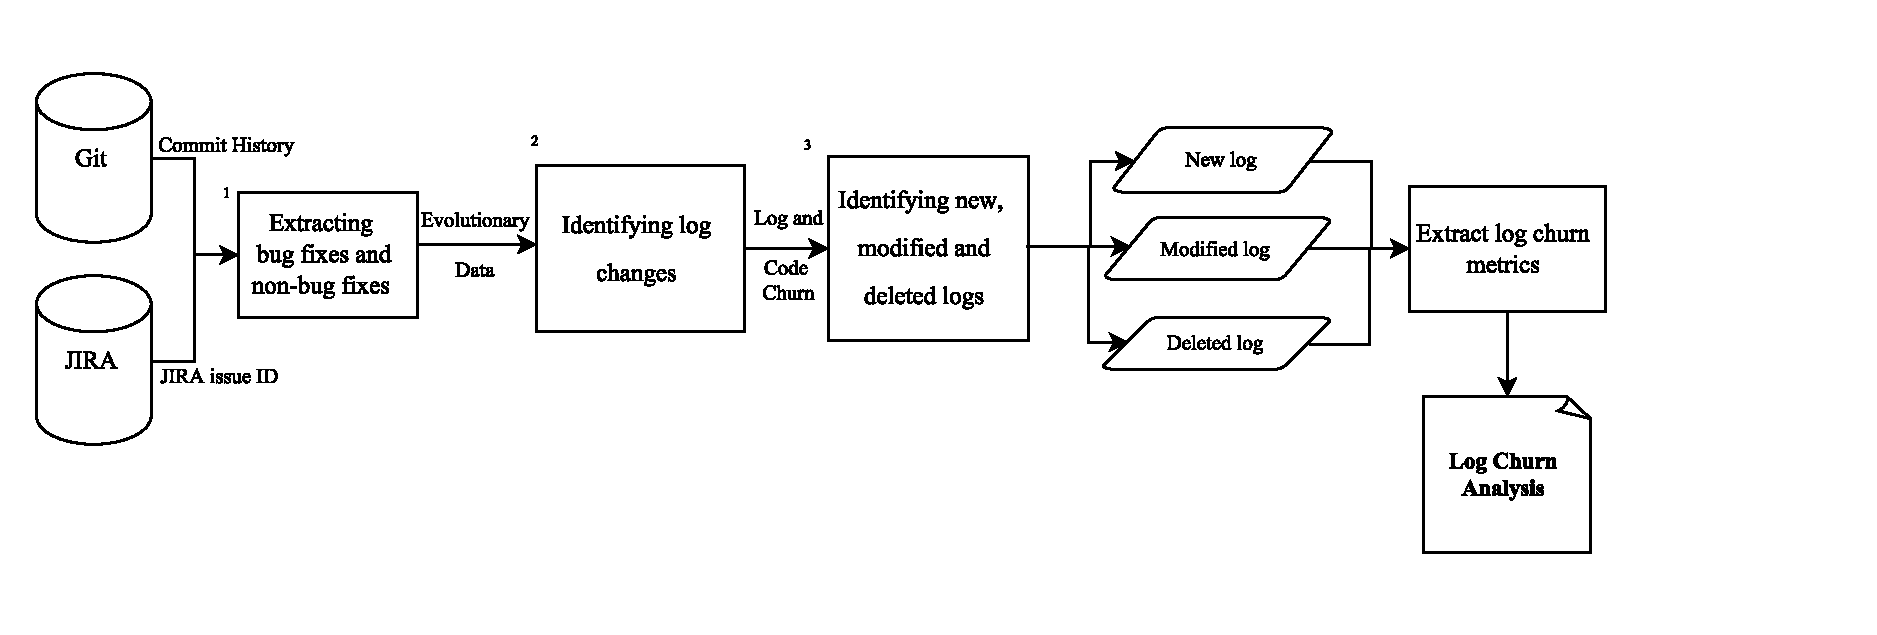
\includegraphics[scale=0.45]{MethdologyICESEM}
	\caption{Overview of our case study approach }
	\label{fig:MethodologyICSME}
\end{figure}

\subsubsection{Extracting bug fixes and non-bug fixes}

The first step in our approach is to extract commits that are associated with bug fixes and the ones that are not associated with bug fixes. First, we extract a list of all commits from the git repository of each project. To avoid the branching and merging commits, we enable the `no-merges' option in the git \textsl{log} command. This flattens all the changes that are made to file in different branches and excludes the final merge between branch and trunk. We also filter out the changes to non-Java files or the test files from the commits. 

Next, we extract a list of all the JIRA issues that have the type \emph{bug}. Developers often mention the JIRA issue ID's in the commit messages. We search JIRA issue IDs in the commit messages to identify all the bug fixes. We exclude commits that do not contain any JIRA ID since we cannot identify if the commit is a bug fix or not. 

\subsubsection{Identifying log changes}

To identify the log changes in the datasets, we first manually explore logs in the source code. Some logs are specific to a particular project. For example, a log from Qpid invokes `QPID\_LOG' to print logs as follows: 
\hypobox{QPID\_LOG(error, ``Rdma: Cannot accept new connection (Rdma exception):
	'' + e.what());
	}

Some logs leverage logging libraries to print logs. For example, \textsl{Log4j}\footnote{http://logging.apache.org/log4j/1.2/} is used widely in \emph{Hadoop} and \emph{HBase}. In both projects, logs have a method invocation `LOG', followed by a logging level. The following log uses \textsl{Log4j}:
\hypobox{ LOG.debug(``public AsymptoticTestCase(String''+ name +``) called'')}

Using regular expressions to match these logs, we automate the process of finding all the logs in the studied projects.


\subsubsection{Identifying new, modified and deleted logs}

Since git \textsl{diff} does not track modification to the code, modifications to a log is shown as a deletion followed by an addition. To track these added and deleted logs we used Levenshtein ratio~\cite{Levenshtein2}. For every pair of added or deleted logs in a commit, we compare the text in parenthesis after removing the logging method (e.g, LOG ) and the log level (e.g, info). We calculate the Levenshtein ratio between the added and deleted log similar to prior research~\cite{levenshteinratio}. We consider a pair of added and deleted logs as a log modification if they have a Levenshtein ratio of 0.6 or higher. For example, the logs shown below have Levenshtein ratio of 0.86. Hence such a pair of added and deleted logs are categorized as a log modification.  
\hypobox{+      LOG.debug(``Call: " +method.getName()+`` took "+ callTime + ``ms");\\ 
	-        LOG.debug(``Call: " +method.getName()+ `` " + callTime);} 

If an added log has a Levenshtein ratio higher than 0.6 with more than one deleted log, we consider the pair of added and deleted logs with the highest Levenshtein ratio as a log modification. After identifying all log modifications, we identify three types of log changes in a commit namely `new logs', `deleted logs' and `modified logs'.



\section{Study Results}
\label{sec:Study}
	In this section, we present our case study results by answering our three research questions. For each research question, we discuss the motivation behind it, the approach to answering the research question and finally the results.

\subsection*{RQ1: Are logs changed more often during bug fixes?}


\subsubsection*{\textbf{Motivation}}

Prior research finds that up to 32\% of the changes to logs are due to field debugging~\cite{EMSEIAN}. During debugging, developers may change logs to gain more run-time information about their system. These log changes may also assist developers in resolving future occurrences of a similar bug. However, to the best of our knowledge, there exists no large scale empirical study to show whether logs are changed more often during bug fixes than other development activities. In addition, we want to investigate how logs are changed during the bug fixes. These findings would provide more insight into what developers consider as important knowledge during bug fixes.

\subsubsection*{\textbf{Approach}}

%Its intuitive that logs are generally modified when bugs are fixed.
%This is because prior research has already proved that a module
%that has been modified continually, has higher chance
%of having bugs than modules which have not been modified \cite{Khosh}.
%So,
We compare the number of changes to logs between bug fixes and non-bug fixes. In previous section, we identified three categories\ian{or types, choose one word across the paper} of logs changes in a commit, i.e., modified, new and deleted logs. Therefore, we compare the number changes to logs within the three types in bug fixes and non-bug fixes. Since commits with higher total code churn may have a higher number of changes to logs, we calculate total code churn for every commit and use it to normalize \emph{\# modified, \# new} and \emph{\# deleted logs}, similar to prior study~\cite{Characterizinglogs}. The three new metrics are:\ian{I rename all the log churn metrics as densities, check across the paper to make sure the naming is consistent.}
\begin{equation}
Modified\ logs\ density = \frac{\#\ of modified\ logs}{\ code\ churn } 
\label{eq1}
\end{equation}
\begin{equation}
New\ logs\  density = \frac{\#\ of new\ logs}{\ code\ churn } 
\label{eq2}
\end{equation}
\begin{equation}
Deleted\ logs\ density = \frac{\#\ of deleted\ logs}{\ code\ churn }
\label{eq3} 
\end{equation}

 %Log density is defined as the ratio of total log churn over total code churn across all commits, as used in prior research. We follow the same approach and find log density of each type of log change for bug fixes and non-bug fixes.

To future understand how logs are modified during bug fixes, we perform a manual analysis on the modified logs to identify the different types of log modifications. We first collect all the commits that modify logs. We select a random sample of 357 commits. The size of our random sample achieves a 95\% confidence level and 5\% confidence interval. We follow an iterative process, similar to prior research~\cite{seaman1999qualitative}, to identify the different types of log modifications, until we cannot find any new types of modifications. 

After we identify the types of log modifications, we create an automated tool to label log modifications into the identified types. We calculate the number of log modifications of every type in each commit and normalize the normalize by {\em code churn}, similar to Equation~\ref{eq1} to \ref{eq3}. We call such metrics of log changes, i.e., modified, new, deleted logs density and the densities of each type of log modifications, as log churn metrics.
%used  as the controlling measure 

We would like to find out whether logs are changed more during bug fixes than non-bug fixes and to identify the type of log change that developers favor during bug fixes. We first compare the mean value of each log churn metric in bug fixes and non-bug fixes by calculating the ratio between the mean value of each log churn metric in bug fixes and non-bug fixes for every studied project. We further compare the log churn metrics by studying whether there is a statistically significant difference in these metrics, between bug fixes and non-bug fixes. We leverage the \textsl{MannWhitney U test} (Wilcoxon rank-sum test)~\cite{Gehan1965}, since our metrics are highly skewed. The {\em MannWhitney U test} is a non-parametric test, such that it does not have any assumptions about the distribution of the sample population. A p-value of \ensuremath{\le} 0.05 means that the difference of the log churn metrics between the bug fixes and non-bug fixes is statistically significant and we may reject the null hypothesis. By rejecting the null hypothesis, we can accept the alternative hypothesis, which tells us that there is a statistically significant difference for our metrics between bug fixes and non-bug fixes.

%and if we use standard T-test the
%resulting p-value will be wrong. {\em Wilcoxon test} is a non-parametric
%test, meaning the distribution of the population does not factor into
%the results.

We also calculate the {\em effect sizes} in order to quantify the differences in log churn metrics between the bug fixes and non-bug fixes. Unlike the {\em MannWhitney U test}, which only tells us whether the difference between the two distributions is statistically significant, the effect size quantifies the difference between the two distributions. Researchers have shown that reporting only the statistical significance may lead to erroneous results (i.e., if the sample size is very large, the p-value are likely to be small even if the difference is trivial). We use {\em Cohen's d} to quantify the effect size~\cite{cohenUsage1,cohenUsage2}. {\em Cohen's d} is defined as:
\begin{equation} \text{{\em d}} = \frac{\bar{x}_1 - \bar{x}_2}{s},
\label{eq:cohensd}
\end{equation}
where $\bar{x}_1$ and $\bar{x}_2$ are the mean of two populations, $s$ is the pooled standard deviation and $d$ is \emph{Cohen's d}~\cite{shadish2009combining}. We use the following thresholds for {\em Cohen's d}~\cite{Effectsize}:
%As software engineering has different thresholds for {\em Cohen's d}~\cite{Effectsize}, the new scale is shown below.

 \begin{align}\label{cohens-d_interpretation-se}
\begin{cases}
\text{trivial}		& \text{for $d \le 0.17$}		\\
\text{small}		& \text{for $0.17 < d \le 0.6$}	\\
\text{medium}	& \text{for $0.6 < d \le 01.4$}	\\
\text{large}		& \text{for $d > 1.4$}
\end{cases}
\end{align}



%\begin{table}[t]
%	\protect\caption{Comparing the mean log density between bug fixes and non-bug fixes (the value of 1.9 for Hadoop means logs are modified 1.9 times more during bug fixes compared to non-bug fixes).}
%	\begin{tabular}{|l|lll|}
%		\hline 
%		\multirow{1}{*}{Projects} & \multicolumn{1}{c}{Modified log density ratio} & \multicolumn{1}{c}{New log density ratio} & \multicolumn{1}{c|}{Deleted log density}\tabularnewline
%		\hline 
%		\multirow{1}{*}{Hadoop} & 1.9 & 1.4 & 1.6\tabularnewline
%		%		\hline 
%		\multirow{1}{*}{HBase} & 3.5 & 1.2 & 2.4\tabularnewline
%		%		\hline 
%		\multirow{1}{*}{Qpid} & 4.1 & 1.2 & 0.5\tabularnewline
%		\hline 
%	\end{tabular}
%	\label{tba:logdensityNewLogs}
%\end{table}

\begin{table}[t]
	\protect\caption{Comparing the mean values of each log churn metric between bug fixes and non-bug fixes. The value of 1.9 for Hadoop means logs are modified 1.9 times more during bug fixes compared to non-bug fixes in Hadoop.}
	\centering
	\begin{tabular}{|l|lll|}
		\hline 
		\multirow{2}{*}{Average ratio of $\frac{Bug\ fixes}{Non-bug\ fixes}$} & \multicolumn{3}{c|}{Projects} \tabularnewline
		 & \multicolumn{1}{c}{Hadoop} & \multicolumn{1}{c}{HBase} & \multicolumn{1}{c|}{Qpid}\tabularnewline
		\hline 
		\multirow{1}{.3\textwidth}{Modified logs density} & 1.9 & 3.5 & 4.1\tabularnewline
		%		\hline 
		\multirow{1}{*}{New logs density} & 1.4 & 1.2 & 1.2\tabularnewline
		%		\hline 
		\multirow{1}{*}{Deleted logs density} & 1.6 & 2.5 & 0.5\tabularnewline

		\multirow{1}{*} {Log relocation density} & 2.0 & 3.3 & 4.9\tabularnewline

		\multirow{1}{*}{Text modification density} & 2.5 & 6.5 & 11.1\tabularnewline
	 			
		\multirow{1}{*}{Variable modification density} & 2.0 & 1.7 & 4.4\tabularnewline

		\multirow{1}{*}{Logging level change density} & 4.0 & 7.5 & 15.8\tabularnewline

		\multirow{1}{*}{Variable addition density} & 2.7 & 1.3 & 25.5\tabularnewline

		\multirow{1}{*}{Variable deletion density} & 2.6 & 1.6 & 4.6\tabularnewline

		\multirow{1}{*}{Variable modification density} & 2.9 & 0.8 & 4.7\tabularnewline
			\hline 				
	\end{tabular}
	\label{tba:logdensityNewLogs}
\end{table}





%\begin{table}[t]
%	\protect\caption{Comparing the mean log density between bug fixes and non-bug fixes. }
%	
%	\centering
%	\begin{tabular}{|>{\centering}p{.15\textwidth}|>{\centering}p{.15\textwidth}|>{\centering}p{.15\textwidth}|>{\centering}p{.15\textwidth}|>{\centering}p{.15\textwidth}|}
%		\hline 
%		\multirow{1}{*}{Projects} & Log relocation density ratio & Text modification density ratio & Variable modification density ratio & Logging level density ratio\tabularnewline
%		\hline 
%		\multirow{1}{*}{Hadoop} & 2.0 & 2.5 & 2.0 & 4.0\tabularnewline
%		%		\hline 
%		\multirow{1}{*}{HBase} & 3.3 & 6.5 & 1.7 & 7.5\tabularnewline
%		%		\hline 
%		\multirow{1}{*}{Qpid} & 4.9 & 11.1 & 4.4 & 15.8\tabularnewline
%		\hline 
%	\end{tabular}
%\end{table}
%



\begin{table}[tbh]
	\caption{Comparing log churn metrics between the bug fixes and non-bug fixes. The p-value is from MannWhitney U tests and the effect sizes are calculated using Cohen's d. A positive effect size shows that the log changes are more frequent during bug fixes.\ian{no need to bold p-value if all of them are bold.}}
	\label{tab:logchange} 
	\centering{}%
	\begin{tabular}{|>{\centering}p{.13\textwidth}|>{\centering}p{.1\textwidth}|>{\centering}p{.1\textwidth}|>{\centering}p{.12\textwidth}|>{\centering}p{.1\textwidth}|>{\centering}p{.1\textwidth}|>{\centering}p{.1\textwidth}|}
		\hline 
		\multirow{2}{*}{Metrics}& \multicolumn{2}{c|}{Hadoop} & \multicolumn{2}{c|}{HBase} & \multicolumn{2}{c|}{Qpid}\tabularnewline
		\cline{2-7} 
		
		& P-values & Effect size & P-values & Effect size & P-values & Effect size\tabularnewline
		\hline 
		Modified log density & \textbf{2.0e-12} & 0.246 (small) & \textbf{1.9e-15} & 0.273 (small) & \textbf{1.6e-11} &  0.432 (small)\tabularnewline
		\hline 
		New log density& \textbf{ 4.7e-16} &  0.265 (small) & \textbf{$<$2.2e-16} & 0.215 (small) & \textbf{ 2.1e-11} & 0.474 (small)\tabularnewline
		\hline 
		Deleted log density& \textbf{8.1e-07} & 0.336 (small) & \textbf{4.9e-07} & 0.150 & \textbf{0.041} & -0.193 (small)\tabularnewline
		\hline 
	\end{tabular}
	
\end{table}

\subsubsection*{Results}
\ian{PLEASE.... make sure the metric names are exactly the same across the paper, in figures, in text and in tables. I corrected some, but please double check them.}
\textbf{Developers are more likely to add new logs when fixing bugs.} From Table~\ref{tba:logdensityNewLogs}, we find that the mean of new log density is 1.2-1.4 times in bug fixes to non-bug fixes. This shows that new logs are 20\%-40\% more likely to occur in bug fixes that non-bug fixes. Table~\ref{tab:logchange} shows that $new\ log\ density$ in bug fixes is higher than non-bug fixes in all studied systems (statistically significant with non-trivial effect sizes). This suggest that developers may need additional information during bug fixes and they add new logs to help fix bugs.
%
%This suggests that developers add new logs during bug fixes than non bug fixes. We find that effect size of new log ratio is higher in \emph{Qpid} than \emph{Hadoop} and \emph{HBase}. This may be because the new log ratio of bug fixes, is three times that of non-bug fixes in \emph{Qpid}. In \emph{Hadoop} and \emph{HBase} we find new log ratio of bug fixes to be only twice that of non-bug fixes. This may be because \emph{Qpid} being a relatively newer system, some important source code may not be well logged. Therefore, developers may have to add additional logs to assist in bug fixes and improve code quality~\cite{EMSEIAN}.

\textbf{Developers are less likely to remove logs during bug fixes.} We find that although the difference of $deleted\ log\ density$ between bug fixes and non-bug fixes is statistically significant in all projects, the effect sizes is trivial for \emph{HBase} and negative for \emph{Qpid} (see Table~\ref{tab:logchange}). Moreover, we find that the log density varies between $0.5$ and $2.4$. This suggests \ian{that... you misses the word ``that'' a lot as grammar issues. please check across the paper.} developers are more likely to remove logs during bug fixes in \emph{Qpid}. Such results confirm the findings from prior research that deleted logs do not have a strong relationship with code quality~\cite{IANEMSE}. 


\begin{table}[t]
	\caption{Distribution of four types of log modifications.}	
	\label{tab:dist}
	\centering
	\begin{tabular}{|>{\centering}p{2.2cm}|>{\centering}p{1.3cm}|>{\centering}p{1.3cm}|>{\centering}p{1.3cm}|}
		\hline 
		Projects & \multicolumn{1}{c|}{Hadoop (\%)} & \multicolumn{1}{c|}{HBase (\%)} & \multicolumn{1}{c|}{Qpid (\%)}\tabularnewline
		\hline 
		Log relocation density  & 73.1 & 70.7 & 47.4\tabularnewline
		\hline 
		Text modification density & 10.5 & 13.4 & 16.8\tabularnewline
		\hline 
		Variable modification density & 9.9  & 10.1 & 18.9\tabularnewline
		\hline 
		Logging level change density& 6.5 & 5.8  & 16.8\tabularnewline
		\hline 
	\end{tabular}
\end{table}

\ian{also check whether you still say logging statements somewhere (except in intro)}
\textbf{Logs are more likely to be modified in bug fixes and non-bug fixes}. From Table~\ref{tba:logdensityNewLogs} we find that on average logs are $1.9$ to $4.1$ times more likely to be modified during bug fixes than non bug fixes. Table~\ref{tab:logchange} shows that $modified\ log\ $ 
$density$ in bug fixes is higher than non-bug fixes in all studied systems (statistically significantly with non-trivial effect sizes). Such results show that developers often modify the information provided by logs to assist in bug fixes. Developers may need different information to the information that is provided by the logs to fix bugs. Prior research find that 66 \% of the logs are modified when 1) the condition that the log depends on is changed, 2) the logged variable is changed or 3) the function name that is also referred in static text of log is modified~\cite{Characterizinglogs}. Therefore, we further explore the different types of modifications to logs.

We manually examine the different modifications to logs and categorize the modifications into four types as follows:
\begin{enumerate}
	\item \textbf{Log relocation:} The log is not changed but moved to a different place in the file.
	\item \textbf{Text modification:} The text that is printed in the logs is modified.
	\item \textbf{Variable change:} One or more variables in the logs are changed (added, deleted or modified).
	\item \textbf{Logging level change:} The verbosity level of logs are changed.
\end{enumerate}
Table~\ref{tab:dist} shows the distribution of each type in our studied systems. When there is co-occurrence of different types of log modifications in a single log, we consider that as new log because it is difficult to categorize all the different types of co-occurrences. \ian{but your new log was defined by levenstain, so did you treat both as new log or what? this is very hard to convince people. I mean, technically, a log modification can be in different types at the same time.}


\textbf{Developers modify logged variables during bug fixes}. From Table~\ref{tba:logdensityNewLogs} we find that variables in logs are $1.7$ to $4.4$ times more likely to be modified during bug fixes. We find that changes to the logged variables are more likely to happen in bug fixes than non-bug fixes (statistically significant with medium or small effect sizes, see Table~\ref{tab:logmod}). This suggests that developers change the logged variables in order to provide useful information in the logs. Prior research also shows that 16-32\% of log changes are made during field debugging~\cite{EMSEIAN}. Therefore, to better understand how developers change logged variables during bug fixes, we categorize the changes into three types: a) variable addition, b) variable deletion and c) variable modification.


\begin{table}[t]
	\protect\caption{Comparing metrics about different types of log modification between bug fixes and non-bug fixes. The p-value are calculated from MannWhitney U tests and the effect sizes are calculated using Cohen's d. A positive effect size shows that the log changes are more frequent during bug fixes. P-values that are smaller than 0.05 are in bold font.\ian{metric names don't match}}
	\label{tab:logmod}
	\centering{}%
	\begin{tabular}{|>{\centering}p{.13\textwidth}|c|>{\centering}p{.1\textwidth}|c|>{\centering}p{.1\textwidth}|c|>{\centering}p{.1\textwidth}|}
		\hline 
		\multirow{2}{*}{Metrics}& \multicolumn{2}{c|}{Hadoop} & \multicolumn{2}{c|}{HBase} & \multicolumn{2}{c|}{Qpid}\tabularnewline
		\cline{2-7} 
		& P-values  & Effect sizes & P-values  & Effect sizes & P-values  & Effect sizes\tabularnewline
		\hline 
		Relocation of log & \textbf{1.1e-10} & 0.330 (small) & \textbf{3.0e-11} & 0.170 (small) & \textbf{1.8e-08} & 0.700 (medium)\tabularnewline
		\hline 
		Modification to logging text & 0.344 & - & \textbf{0.0075} & 0.525 (small) & \textbf{4.5e-06} & 0.976 (medium)\tabularnewline
		\hline 
		Modification of logged variable  & \textbf{1.3e-04} &0.351 (small) & \textbf{0.0010} & 0.420 (small) & \textbf{1.2e-04} &  1.17 (medium)\tabularnewline
		\hline 
		Modification to logging level &  0.108 & - & 0.503 & - & 0.399 & - \tabularnewline
		\hline 
	\end{tabular}
\end{table}



\begin{table}[t]
	\caption{Comparing the different types of changes to variables between the bug fixes and non-bug fixes. A positive effect size shows that the log changes are more frequent during bug fixes. P-values that are smaller than 0.05 are in bold font.\ian{metric names don't match}}
	\label{tab:varmod}
	\centering
	\begin{tabular}{|>{\centering}p{.13\textwidth}|c|>{\centering}p{.1\textwidth}|c|>{\centering}p{.1\textwidth}|>{\centering}p{.1\textwidth}|p{0.1\textwidth} |}
		\hline 
		\multirow{2}{*}{Metrics}& \multicolumn{2}{c|}{Hadoop} & \multicolumn{2}{c|}{HBase} & \multicolumn{2}{c|}{Qpid}\tabularnewline
		\cline{2-7} 
		& P-values  & Effect sizes & P-values  & Effect sizes & P-values  & Effect sizes\tabularnewline
		\hline  Variable addition & 0.099  & -  & \textbf{0.00049}& 0.659 (medium) & \textbf{0.005}& 1.40 (large) \\ 
		\hline  Variable deletion & 0.098 &   - & 0.355 & -  & 0.193 & -  \\ 
		\hline Variable modification & \textbf{4.11e-05} & 1.045 (medium)  & 0.568 & - & \textbf{0.0016}& 0.949 (medium)   \\ 
		\hline 
	\end{tabular} 
\end{table}

Table~\ref{tab:varmod} shows that developers modify the logged variables more in bug fixes than non-bug fixes (statistically significant with medium effect sizes). This modification may be because developers need different information rather than the information provided by existing logs. For example, when manually exploring the patch notes for bug QPID-2370\footnote{https://issues.apache.org/jira/browse/QPID-2370}, we find that developers modify the existing log to capture a newly defined variable. The other reason may be that developers change the name of the existing variable to a more meaningful name. For example, in bug MAPREDUCE-2264\footnote{https://issues.apache.org/jira/browse/MAPREDUCE-2264}, we find that developers rename variables and modify the logs accordingly. %Prior research also find that developers often have after-thoughts on logs~\cite{Characterizinglogs}.

From Table~\ref{tab:varmod}, we observe that the developers add variables more in bug fixes than non-bug fixes (statistically significant with medium effect size in \emph{HBase} and large effect size in \emph{Qpid}). We find from Table~\ref{tba:logdensityNewLogs} that developers are $1.3$ to $25.2$ times more likely to add new variables during bug fixes than non-bug fixes. This addition of variables suggests that existing variables may not have all the needed information in the logs and developers have to add new variables during bug fixes. We also find that developers do not delete variables in logs. Deleting variables in logs may change the format of logs. There may be log processing tools\ian{tools or applications make consistent across} that rely on these logs. Deleting variables may impact the correctness of these log processing applications\ian{applications or tools}~\cite{IanWCRE}. Therefore, developer may be aware of the such impact and try to avoid deleting variables from logs.
 
 
\textbf{Developers modify logged text more during bug fixes.} We find that modification of logged text is more likely to happen in bug fixes than non-bug fixes with non-trivial effect sizes (see Table~\ref{tab:logmod}). In some cases, the text description in logs is not clear and developers need to improve the text. For example, to fix bug HBASE-6665\footnote{https://issues.apache.org/jira/browse/HBASE-6665} developers modify a log to provide a better description of the operation. Prior research shows that up to 39\% of modifications to logged text is due to inconsistency between the execution event and the message conveyed by logs~\cite{Characterizinglogs}. Our results suggest that developers may have faced such challenges during bug fixes and may modify the text in logs for better description. 
%'

%that developers value more in providing contextual data to an existing
%log rather than writing new logs. 

\textbf{Log relocation occurs more in bug fixes.} Table~\ref{tab:dist}, shows that there are a large number of log changes that only relocate logs. Table~\ref{tab:logmod} shows that such relocation of logs is statistically significantly more in bug fixes than non-bug fixes ($2.0$ to $4.9$ times more likely in bug fixes as shown in Table~\ref{tba:logdensityNewLogs}). We manually examine such commits and find that developers often forget to leverage exception handling or using proper condition statements in the code. After fixing the bugs, developers often move existing logs into the \emph{try/catch} blocks or after condition statements. For example, to fix bug YARN-289 \footnote{https://issues.apache.org/jira/browse/YARN-289} from Hadoop, logs are placed into a proper \emph{if-else} block.

\textbf{Logging levels are not modified often during bug fixes.} We find that logging level changes are statistically indistinguishable between bug fixes and non-bug fixes in all the studied systems. The reason may be that developers are able to enable all the logs during bug fixes, despite of what level a log has. In addition, prior research shows that developers do not have a good knowledge about how to choose a correct logging level~\cite{Characterizinglogs}. 


\hypobox{Developers change logs statistically significantly more in bug fixes than non-bug fixes. In particular, developers modify logs to add or change the variables in logs during bug fixes. This suggests that developers often realize the needed information to be logged as after-thoughts and change the variables in log to assist in fixing bugs.}


\subsection*{RQ2: Is there a relationship between log changes and effort spent on bug fixes?}


\subsubsection*{Motivation}

In RQ1, we find that logs are more likely to be changed in bug fixes. However, we do not know whether changing logs has a relationship with effort spent on bug fixes. If changing logs during bug fixes has relationship with the effort of bug fixes, developers may consider leveraging and improving logs during bug fixes in order to save effort.

\subsubsection*{Approach}


To answer the research question, 

To study whether there is a relationship between effort spent on bug fixes and changing logs during bug fixes, we collect all JIRA issues with type \emph{bug} from the three studied systems. We obtained the code commits for each of these JIRA issues by searching for the issue id from commit messages. We then separate the JIRA issues into (1) bugs that are fixed with log churn and (2) bugs that are fixed without log churn. We calculate the log churn metrics for each bug. If a issue has multiple commits we calculate the log churn metrics for each commit individually. We then measure effort of bug fixes using the time taken to resolve a bug, the number of developers involved during the resolution of a bug and the number of discussion posts about the bug on JIRA. Prior research has shown that such metrics are good estimates of developer effort~\cite{amor2006effort}. 

%:\ian{check the paper that you cite to build a model to predict resolution time to see whether there is any thing you can back up for the choice of these three metrics}
\begin{enumerate}
	\item \textbf{Resolution time:} This metric measures how fast the bug is fixed. This metric is defined as the time taken from when the bug is opened until it is resolved. For example, if a bug was opened on 1$ ^{st}$ February 2015 and closed on 5$ ^{th}$ February 2015, the resolution time of the bug is four days. 
	
	\item \textbf {\# of comments:} This metric measures how much discussion is needed to fix a bug. Intuitively, the more discussion in an issue report, the more effort is spent on fixing the bug. We count the total number of comments in the discussion of each issue report.
	
	\item \textbf {\# of developers:} This metric measures the number of developers who participate in the discussion of fixing the bug. Intuitively, more developers who discuss the bug, more effort is spent on fixing the bug. We count the number of unique developers who comment on the issue report. We use the user names in the JIRA discussion to identify the developers. 
\end{enumerate}
Intuitively, a complex bug fix might have more code churn and in turn takes longer time to be resolved, more developers being involved and more discussions on JIRA. Therefore, we use code churn to normalize the resolution time, the number of comments, and the number of developers during bug fixes. We use these normalized effort metrics to find if there is statistically significant difference between bug fixes with log churn and bug fixes without log churn. We use the {\em MannWhitney U} test to find the $|\rho|$ values and \textsl{Cohen's d} test to measure the effect size, similar to RQ1. 

%We use the code churn to measure the complexity of the issue. 


 %and the code churn for fixing each issue We then extracted three metrics from JIRA issues to measure the effort of fixing a bug:

%Prior research has shown that complexity of software can be measured using different metrics, including source lines of code change~\cite{complexity}. 


\begin{table*}
	\caption{Comparing code and developer metrics between the bug fixes with log churn and bug fixes without log churn.The p-value is from MannWhitney U tests and the effect sizes are calculated using Cohen's d. A positive effect size shows that the code changes are more frequent during bug fixes log churn.}
	\label{tab:bugfixes}
	\centering{}%
	\begin{tabular}{|>{\centering}p{.12\textwidth}|c|>{\centering}p{.1\textwidth}|c|>{\centering}p{.1\textwidth}|c|>{\centering}p{.1\textwidth}|}
		\hline 
		\multirow{2}{*}{Metrics}& \multicolumn{2}{c|}{Hadoop} & \multicolumn{2}{c|}{HBase} & \multicolumn{2}{c|}{Qpid}\tabularnewline
		\cline{2-7} 
		
		& p-values  & Effect size & p-values  & Effect Size & p-values  & Effect size\tabularnewline
		\hline 
		Code churn &  $<$2.2e-16 & 0.178 (small) & $<$2.2e-16 & 0.023 &  $<$2.2e-16 & 0.155\tabularnewline
		\hline 
		Resolution time & 4.7e-14 &  -0.095 & $<$2.2e-16 & -0.188 (small) &  7.7e-08 & -0.276 (small)\tabularnewline
		\hline 
		\# of comments & 2.2e-16 & -0.573 (small) &  $<$2.2e-16 &-0.436 (small) & $<$2.2e-16 & -0.304 (small)\tabularnewline
		\hline 
		\# of developers &  $<$2.2e-16 & -0.539 (small) & $<$2.2e-16 & -0.617 (medium) & $<$2.2e-16 & -0.440 (small)\tabularnewline
		\hline 
	\end{tabular}
\end{table*}
 
 \begin{figure*}[t]
 	\centering
 	\caption{Boxplot of code churn of bug fixes with log churn (shown in blue) against bug fixes without log churn (shown in grey).}
 	\label{fig:figure3}
 	
 	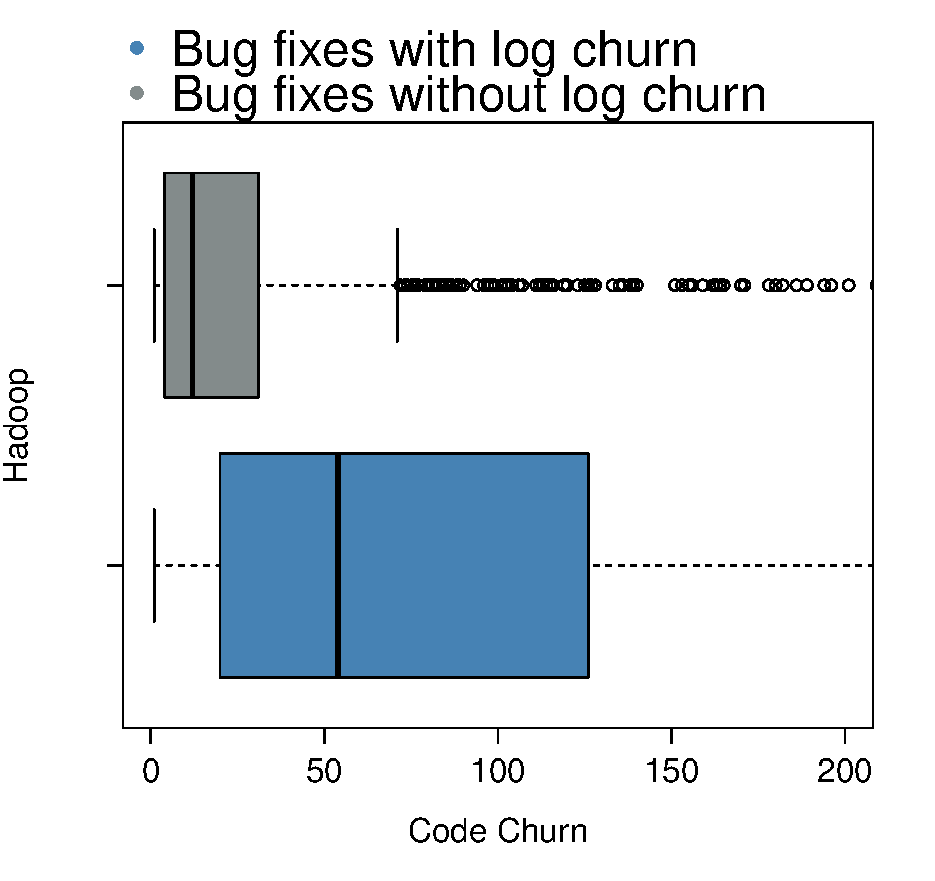
\includegraphics[width=.49\textwidth]{HadoopBoxPlot}
 	\hfill
 	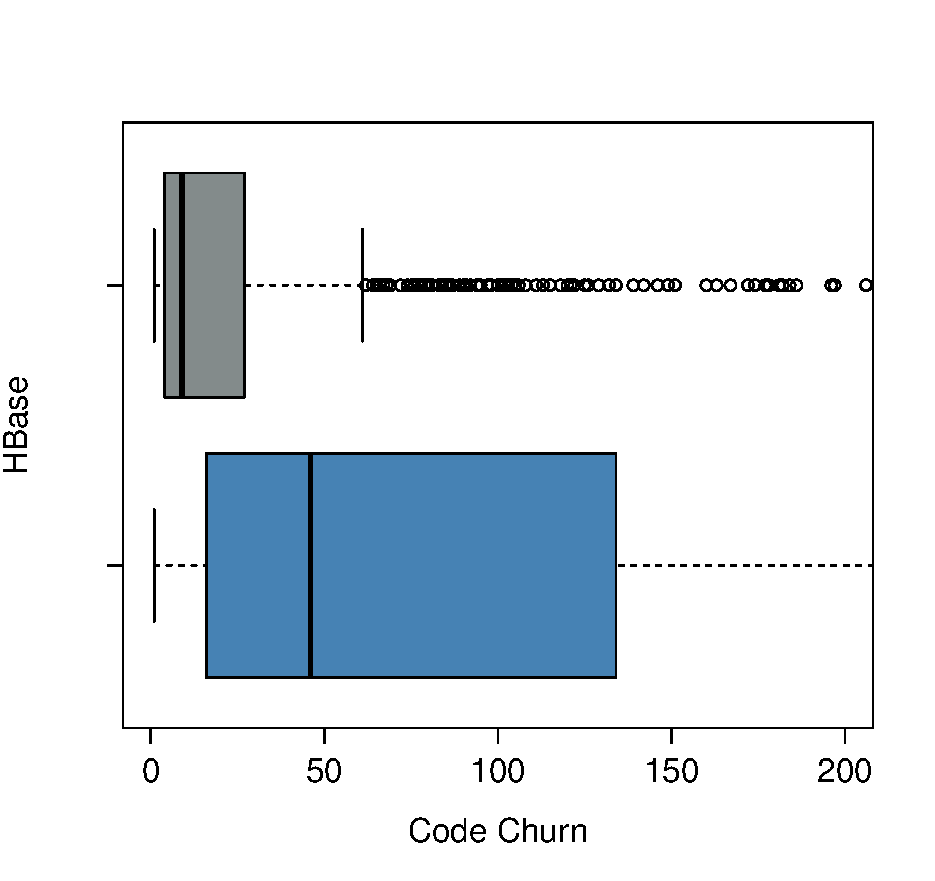
\includegraphics[width=.49\textwidth]{HBaseBoxPlot}\hfill
 	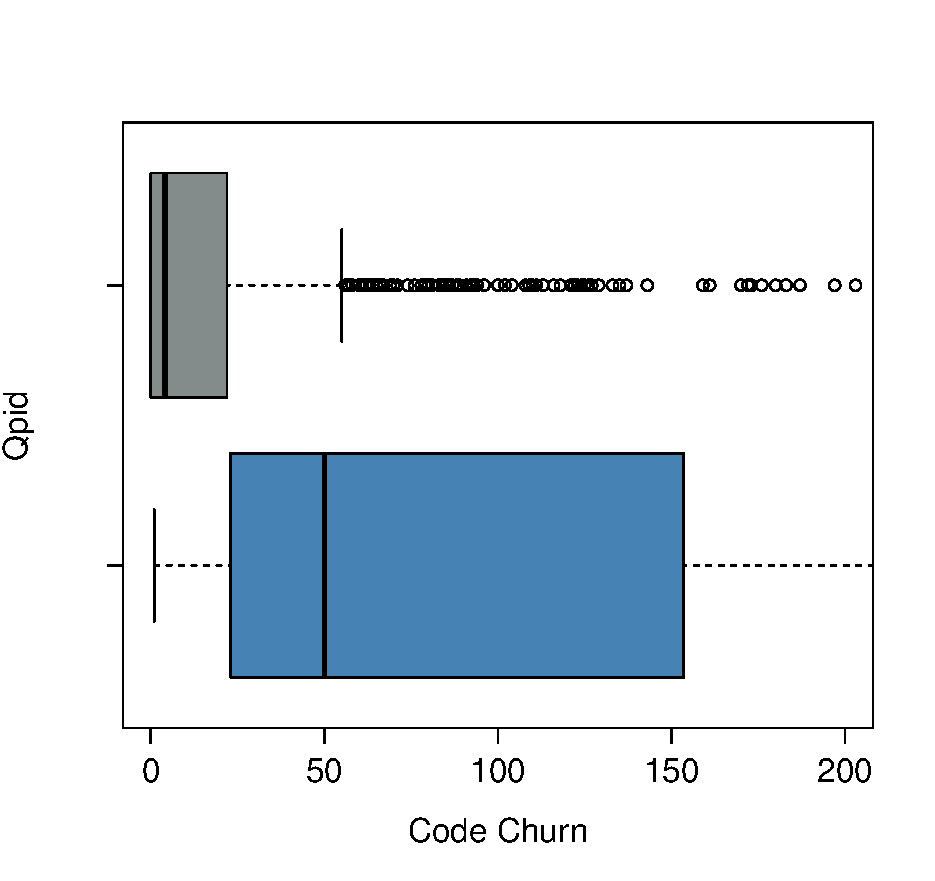
\includegraphics[width=.49\textwidth]{QpidBoxPlot}
 	
 \end{figure*}


\subsubsection*{Results}

\textbf{We find that the log changes are more likely to occur during more complex bugs fixes}. We find that the average code churn for fixing bugs is significantly higher with log churn than without log churn (see Table~\ref{tab:bugfixes} and Figure~\ref{fig:figure3}). This suggests that complex bug fixes are more likely to have log churn (statically significant with non-trivial effect size). 

\textbf{We find that bugs that are fixed with log churn, take shorter time with fewer comments and fewer people.} After normalizing the code churn, we find that the resolution time, the number of comments and the number of developers are all statistically significantly smaller in the bug fixes with log churn than the ones without log churn. This result suggests that given two bugs of the same complexity, the one with log churn is likely to take less time to get resolved and likely to need a fewer number of developers involved with fewer discussions. Changing logs may provide useful information to assist developers in discussing, diagnosing and fixing bugs. For example, when fixing bug HBASE-3074\footnote{https://issues.apache.org/jira/browse/HBASE-30741}, developers left the first comment to provide additional details in the log about where the failure occurs. Developers add the name of the servers into the the logs. Such additional data helps diagnose the cause of the failure and helps fix the bug.

\subsubsection*{Discussion}

To further understand how developers change logs during bug fixes, we conduct a manual analysis. We collected all the bug fixes with log changes for our studied systems. We selected a 5\% random sample (266 for \textsl{HBase}, 268 for \textsl{Hadoop} and 83 for \textsl{Qpid}) from all the commits. For the sampled commits, we manually examine the code changes and the corresponding JIRA issue reports to find the reasons of changing logs during bug fixes. We follow an iterative process, similar to prior research~\cite{seaman1999qualitative}, until we cannot find any new reasons. We find three reasons of changing logs during bug fixes as shown in Table~\ref{tba:LogUsage}. These three reasons may co-occur within a single commit. 

% The code changes are analyzed to identify common patters of log usage during debugging and JIRA issue reports are analyzed to understand the extent of log usage by developers.
\begin{table}[tbh]
	\protect\caption{Log change reasons during bug fix}
	\label{tba:LogUsage}	
	\begin{centering}
		\begin{tabular}{|>{\centering}p{2.5cm}|>{\centering}p{1.3cm}|>{\centering}p{1.3cm}|>{\centering}p{1.3cm}|}
			\hline 
			Projects & Hadoop & HBase & Qpid\tabularnewline
			\hline 
			\hline 
			Bug diagnosis & 157 & 175 & 49\tabularnewline
			\hline 
			Similar bugs detection & 156 & 170 & 42\tabularnewline
			\hline 
			Code quality assurance for bug fixes & 93 & 78 & 18\tabularnewline
			\hline 
		\end{tabular}
		\par\end{centering}
	
\end{table}
\begin{itemize}
	

\item \textbf{Bug diagnosis.} Developers change logs to print extra or different information into logs during the execution of the system. Such information is printed to ease bug diagnosis.
%The log changes in the category have added and deleted code prior to log changes (i.e., code block is changed). 
For example, HADOOP-2725\footnote{https://issues.apache.org/jira/browse/HADOOP-2725} is reported when users find that after copying a 100TB file across two clusters, the file sizes has a discrepancy of 6GB. However, the existing logs do not have proper format to show the size of the copied data. To help diagnose the bug, developers modify the logged variable to print the sizes of the copied data into a better format. %These log changes are committed along with bug fix, as it clarifies the log output and helps in understanding the logging context.

 %These findings are consistent with prior findings where majority of log changes are made during debugging~\cite{EMSEIAN}.

\item \textbf{Similar bugs detection.} After fixing a bug, developers may insert log into the code in order to monitor the execution of the system to detect similar bugs in the future. During the bug fixes, developers identify root-causes of the bug. After fixing the bug, developers change logs to capture the run-time event that may correspond to the root-cause of the bug, in order to identify future occurrence of a similar bug. The changed information in logs is not leveraged to fix the bug, but rather monitoring the systems for detecting a similar bug in the future. We find that logs in this category are mainly new logs being added into the system, unlike bug diagnosis which is mainly log modifications. 
%Log changes in this category have addition of new blocks (i.e., if, if-else, try-catch and exception) with higher code addition than deletion. 
For example, to fix HADOOP-2890\footnote{https://issues.apache.org/jira/browse/HADOOP-2890}, developers identify the reason behind blocks getting corrupted as an run-time exception. In the commit, we observe that the developers fix this bug and add \textsl{try catch} block with new logs to catch these exceptions. Such log will notify developers if a similar bug appears.

\item \textbf{Code quality assurance for bug fixes.} Sometime, developers need to introduce a large amounts of code to fix a bug. The introduction of bug-fixing code, may also introduce new bugs into the system. To ensure the quality of these bug fixes, developers insert new logs into the bug-fixing code. For example, in HBASE-3787\footnote{https://issues.apache.org/jira/browse/HBASE-3787}, developers encounter a non-idempotent operation (i.e., running the operation more than once produces different results) that causes an error in the application. The fix of this bug involves over 13 developers and 112 discussions over the two years. The developers add several new files and functions during the bug fix, and added logs to assure the code quality of the fix. 
\end{itemize}


\hypobox{Logs are more likely to be changed during fixing more complex bugs. After normalizing the complexity of bugs using code churn, we find that bug fixes with log churn are resolved faster with fewer people and fewer discussions.}


%\subsection*{RQ3: Can log churn metrics help in explaining the resolution time of bugs?} 

\subsubsection*{Motivation}
%Prior research has shown that resolution time is correlated to the number of developers and the number of comments in an issue report~\cite{RTpredictions}. However, prior research does not look at the type of changes made by developers. 

In RQ2, we find that bug fixes with log churn take shorter time to get resolved than bug fixes without log churn. However, there may be confounding effects between metrics, i.e., resolution time, total churn, \# of developers and \# of discussions, such that it is difficult to draw unbiased conclusion on the relationship between resolution time and log churn. To further explore this relationship between resolution time and log changes in bug fixes, we build prediction models using metrics from prior research and log churn metrics. %We want to understand the effect of log changes during bug fixes and also identify which types of log changes can be beneficial during bug fixes. 

\subsubsection*{Approach}

To better understand the relationship between log changes and the resolution time for fixing bugs, we build a non-linear regression model. Prior research has shown that linear modelling can help in predicting the resolution time of bugs~\cite{anbalagan2009predicting}. However, the relationship between resolution time of bug fixes and log changes may be non-monotonic. By building a non-linear regression model we can more appropriately approximate the relationship between resolution time and log churn metrics, during bug fixes.

A non-linear regression model fits the curve of the form $y = \alpha + \beta_{1}x_{1} + \beta_{2}x_{x} + .. + \beta_{n}x_{n} $ to the data, where $y$ is the dependent variable (i.e., resolution time of bugs) and every $x_{i}$ is an explanatory metrics. The explanatory metrics include the log churn metrics (as shown in RQ1). Since prior research finds that the number of developers and the number of comments in an issue report are correlated to the resolution time of the issue report, we include the number of developers and the number of comments as explanatory metrics. We find that bugs with more complex fixes may take longer time to resolve (see RQ2). Therefore, we also include code churn as an explanatory metric. We use the \textsl{rms} package~\cite{rmsPackage} from R, to build non-linear regression models. The overview of our modeling process is shown in Figure~\ref{fig:MethodologyOLS} and is explained below. 




% In our model, \textsl{resolution time} is the dependent variable $y$ and the log churn metrics are the explanatory variables.


\noindent \textbf{(1) Calculating the degrees of freedom}

During predictive modeling, a major concern is over-fitting. An over-fit model is biased towards the dataset from which it is built and will not well fit other datasets. In non-linear regression models, over-fitting may creep in when an explanatory metric is assigned more degrees of freedom than the data can support. Hence, it is necessary to calculate a budget of degrees of freedom that a dataset can support before fitting a model. We budget $\frac{x}{15}$ degrees of freedom for our model as suggested by prior research~\cite{DegreesofFreedom}, where \textsl{x} is the number of rows (i.e, \# bugs) in each project. 


\noindent \textbf{(2) Correlation and redundancy analysis}

Correlation analysis is necessary to remove the highly correlated metrics from our dataset. We use Spearman rank correlation to assess the correlation between the metrics in our dataset. We use Spearman rank instead of Pearson correlation because Spearman rank correlation is resilient to data that is not normally distributed. We use the function \textsl{varclus} in R to perform the correlation analysis. From the hierarchical overview of explanatory metrics constructed by the \emph{varclus} function, we exclude one metric from the sub-hierarchies which have correlation $|\rho| > 0.7 $.
% \ian{what's your cutoff and how do you decide which metrics to remove, check what shane wrote.}

Correlation analysis does not indicate redundant metrics, i.e, metrics that can be explained by other explanatory metrics. The redundant metrics can interfere with the one another and the relation between the explanatory and dependent metrics is distorted. We perform redundancy analysis to remove such metrics. We use the \textsl{redun} function that is provided in the \textsl{rms} package to perform the redundancy analysis.

\begin{figure}
	\centering
	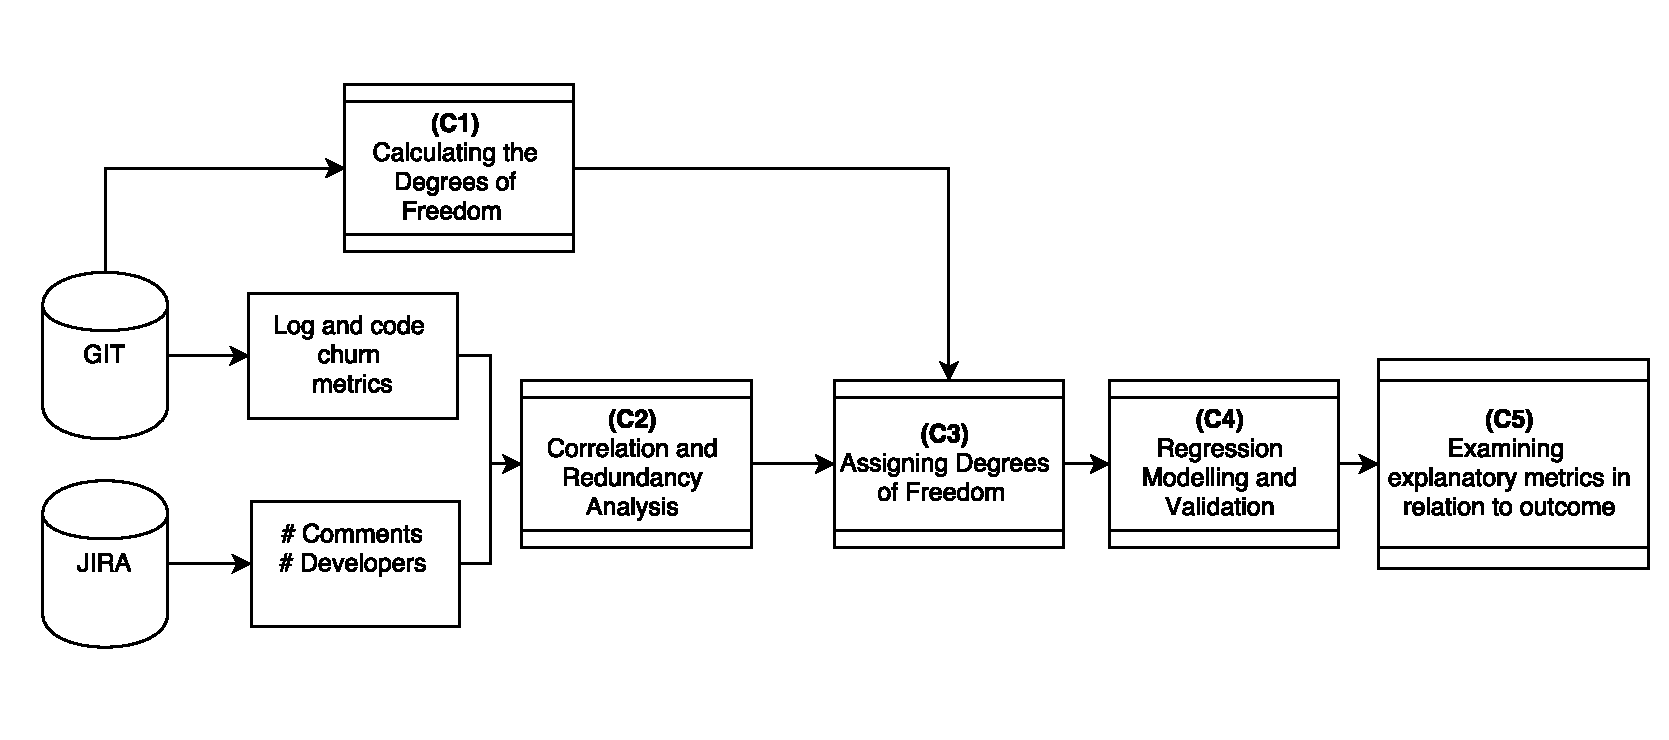
\includegraphics[width=9.8cm]{MethodologyOLS}
	\caption{Overview of our non-linear OLS model construction(C) for the resolution time of bugs}
	\label{fig:MethodologyOLS}
\end{figure}



\noindent \textbf{(3)Assigning degrees of freedom}


After removing the correlated and redundant metrics from our datasets, we spend the budgeted degrees of freedom efficiently. We identify the metrics which can use the benefit from the additional degrees of freedom (knots) in our models. To identify these metrics we use the Spearman multiple $\rho^{2}$ between the explanatory and dependent metrics. A strong relation between explanatory metrics $x_{i}$ and the dependent metric $y$ indicates that, $x_{i}$ will benefit from the additional knots and improve the model. We use the function \textsl{spearman} in the \textsl{rms} package to calculate the Spearman multiple $\rho^{2}$ values for our metrics (metrics with larger $\rho^{2}$ values are allocated more degrees of freedom than metrics with smaller $\rho^{2}$ values).

\noindent \textbf{(4)Regression modeling and validation}

After budgeting degrees of freedom to our metrics we build a non-linear regression model using the function OLS (Ordinary Least Squares) that is provided by the \textsl{rms} package. We use the \textsl{restricted cubic splines} to assign the knots to the explanatory metrics in our model. 
As we are trying to identify the relationship between log churn metrics and the resolution time of bug fixes, we are primarily concerned if the log churn metrics are significant in our models. Therefore, we use chunk test (a.k.a Wald test) to determine the statistically significant metrics to included in our final model. We choose chunk test as some of our explanatory variables are allocated several degrees of freedom and have to be tested jointly, similar to previous research~\cite{ShaneOLS}. At each step in the Wald test, we measure the significance of each metric according to its p-value. We consider only those metrics that have p-values lower than 0.05 in the final model. We use \textsl{wald.test} function provided by the R package \emph{aod}~\cite{waldtest} to perform the chunk test.  


\noindent \textbf{(5) Examining explanatory metrics in relation to outcome}

After identifying the significant metrics in our datasets we find the relation between each explanatory metric and the resolution time of bugs. In our regression models, each explanatory metric can be explained by several knots assigned to that metric. To account for the impact of all knots associated with an explanatory metric, we plot the changes to resolution time against each metric, while holding the other metrics at their median value using the \emph{Predict} function in the \emph{rms} package~\cite{rmsPackage}. The plot follows the relationship as it changes directions at the spline (knot) locations (C-3). 

We would like to point out that although non-linear regression models can be used to build accurate models for the resolution time of bugs, our purpose of using the non-linear regression models in this paper is not for predicting the resolution time of bugs. Our purpose is to study the explanatory power of log churn metrics and explore their empirical relationship to the resolution time of bugs.%We controlled the metrics by total code churn. We used \textsl{Wilcoxon} test to measure the statistical significance of each metric in bugs fixed with log changes with bugs fixed without log changes. \textsl{Cohens.D} is used to measure the size of the difference of each metric. 



\subsection*{Results}

\begin{figure}[t]
	\centering 
	\begin{minipage}[b]{1\columnwidth}
			\centering 
			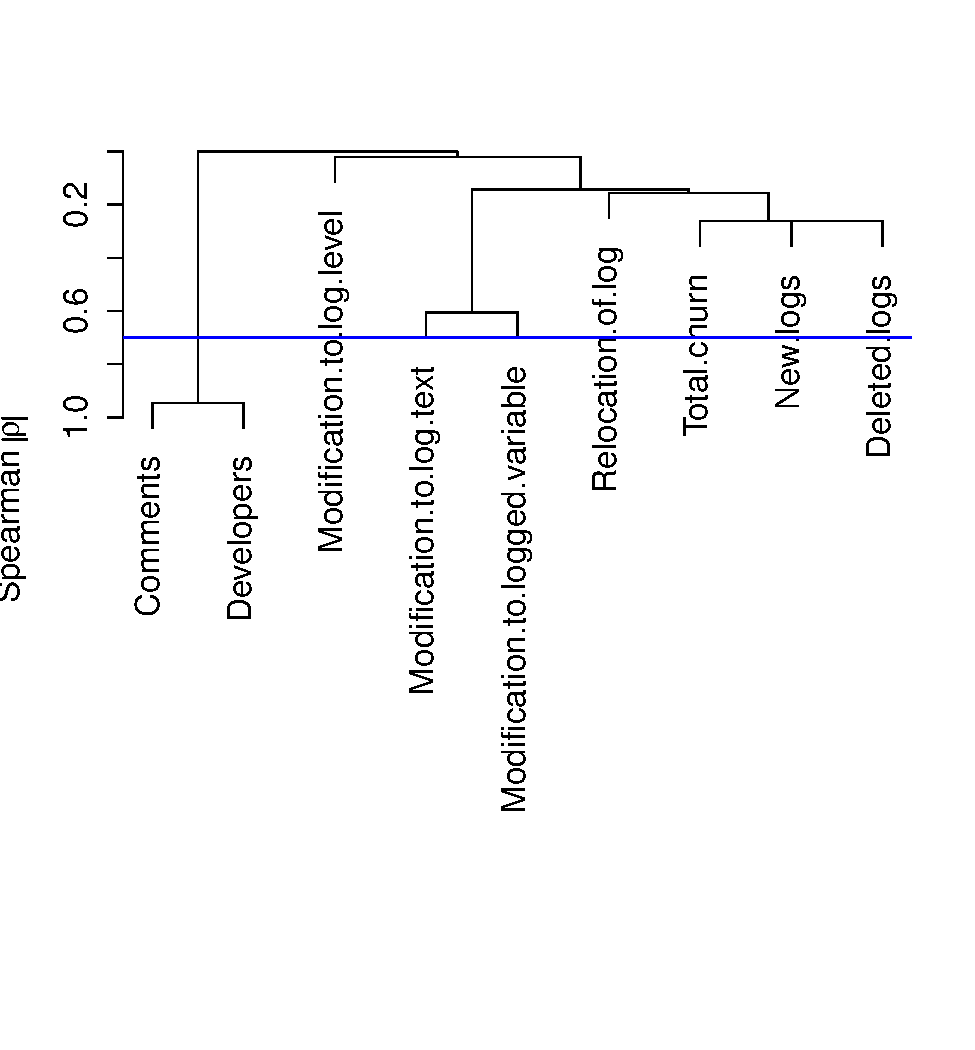
\includegraphics[width=.8\columnwidth]{QpidSpearman}	
		%		\subcaption{Correlation between metrics in Qpid}

	\end{minipage}
	
	\vspace*{-1.5cm}	\caption{Correlation between metrics in Qpid. Blue line indicates cut of set to 0.7\label{fig:Correlation}}
\end{figure}

In this subsection, we describe the outcome of the model construction and analysis outlined in our approach and Figure~\ref{fig:MethodologyOLS}

\textbf{(1) Calculating degrees of freedom}. Our data can support 123 ($\dfrac{1,925}{15}$ in Hadoop), 63($\dfrac{953}{15}$ in Qpid) and 183($\dfrac{2,755}{15} $ in HBase) degrees of freedom for the studied projects. As we have large degrees of freedom in each project, we can be liberal in the allocating splines (knots) to the explanatory variables during model construction. 


\textbf{{(2) Correlation and redundancy analysis}}. Figure~\ref{fig:Correlation} shows the hierarchically clustered Spearman $\rho$ values of the three systems. The blue line indicates our cut-off value ($|\rho|$ = 0.7 ). Our analysis reveals that \# \textsl{Comments} and \# \textsl{developers} are highly correlated in \emph{Qpid} and \emph{HBase}. We chose to remove \#\textsl{developers} from our model since \#\textsl{comments} is a simpler metric than \#\textsl{developers}. We find that there are no redundant metrics in our metrics in all the studied projects.


\textbf{(3) Assigning degrees of freedom}. Figure~\ref{fig:Spearman} shows the Spearman multiple $\rho^{2}$ of the resolution time against each explanatory metric. Metrics that have higher Spearman multiple $\rho^{2}$ have higher chance of benefiting from the additional degrees of freedom to better explain resolution time. Based on Figure~\ref{fig:Spearman}, we split the explanatory metrics into three groups. The first group consists of \#\textsl{comments}, the second group consists of \#\textsl{modifications to log level}, \#\textsl{ modifications to log variable}, \#\textsl{relocation of log} and \#\textsl{new logs}. The last group consists of the remaining metrics. We allocate five degrees of freedom i.e, knots, to the metrics in the first group, three to metrics in second group and no knots to metrics in last group similar to prior research~\cite{ShaneOLS}.


\begin{figure}[t]
	\begin{minipage}[b]{1\columnwidth}
			\centering 
		\hspace*{-2cm}	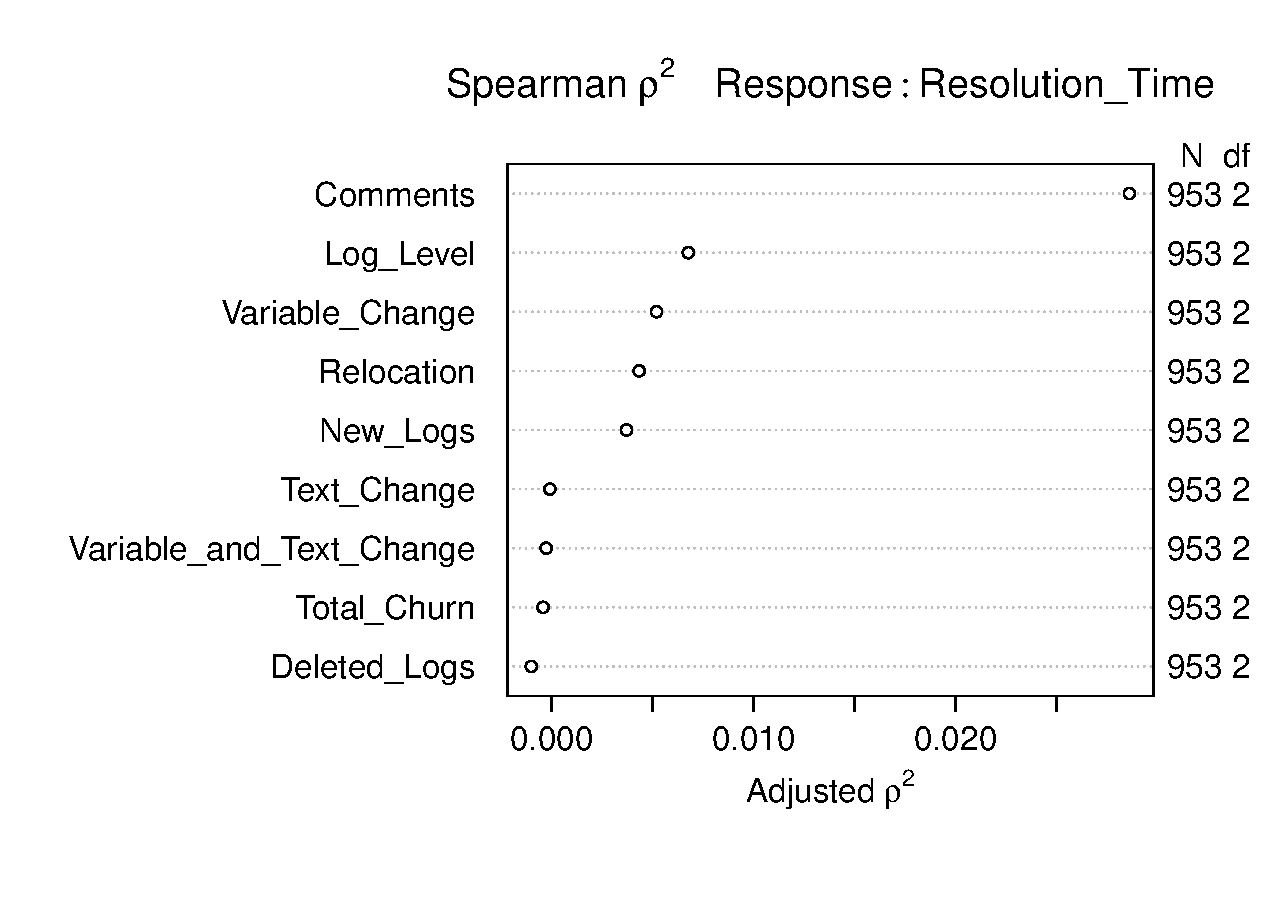
\includegraphics[width=0.7\textwidth]{QpidDF}	
		
	\end{minipage}
	\captionsetup{labelsep = colon}
	\hspace*{1.7cm}\caption{Spearman multiple $\rho^{2}$ of each explanatory metric against Resolution Time of bug fixes with log changes. Larger values indicate more potential for non-linear relationship \label{fig:Spearman}}
\end{figure}




\textbf{(4) Regression modeling and validation.} After allocating the knots to the explanatory metrics, we build the non-linear regression model and use the \textsl{validate} function in the \textsl{rms} package to find the significant metrics in our studied projects. We find that log churn metrics are significant in Qpid and HBase systems for predicting resolution time of bug fixes. 

\begin{figure*}[t]
	\begin{minipage}{.5\columnwidth}
		\centering
		
		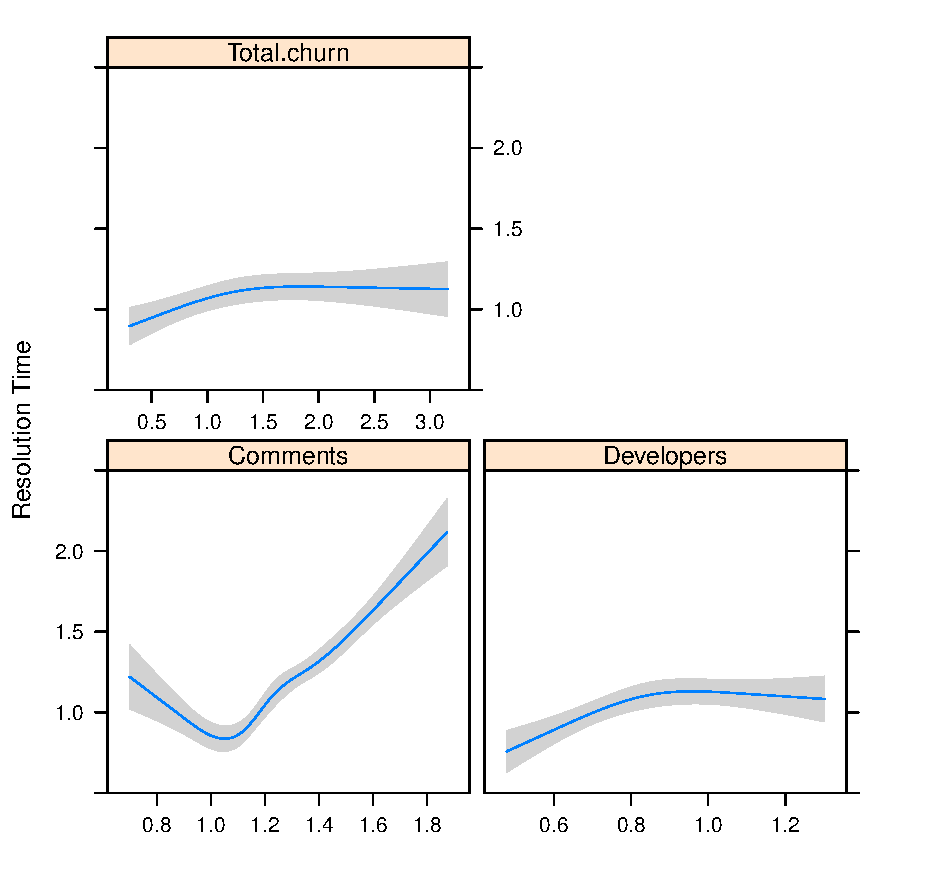
\includegraphics[width=.95\textwidth]{HadoopDirectionPlot}	
		\subcaption{Hadoop}
	\end{minipage}
		\begin{minipage}{.5\columnwidth}
			\centering
			
			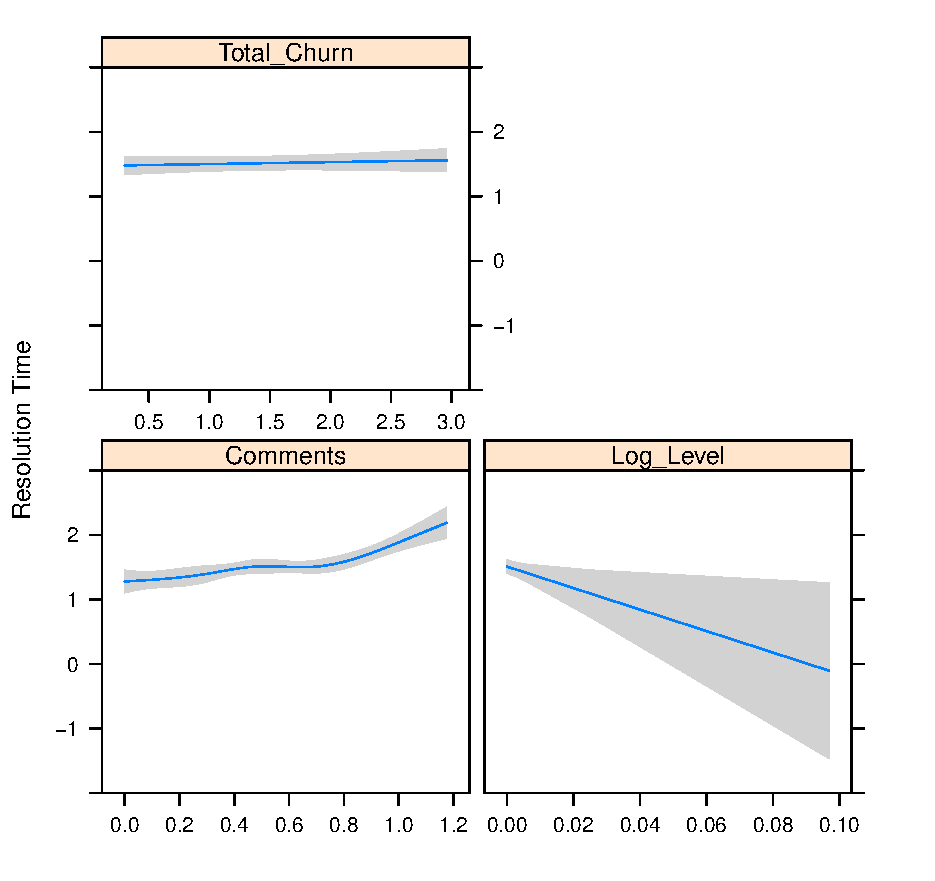
\includegraphics[width=.95\textwidth]{QpidDirectionPlot}	
			\subcaption{Qpid}
		\end{minipage}
			
	\begin{minipage}{0.5\columnwidth}
		\hspace*{1.9cm}	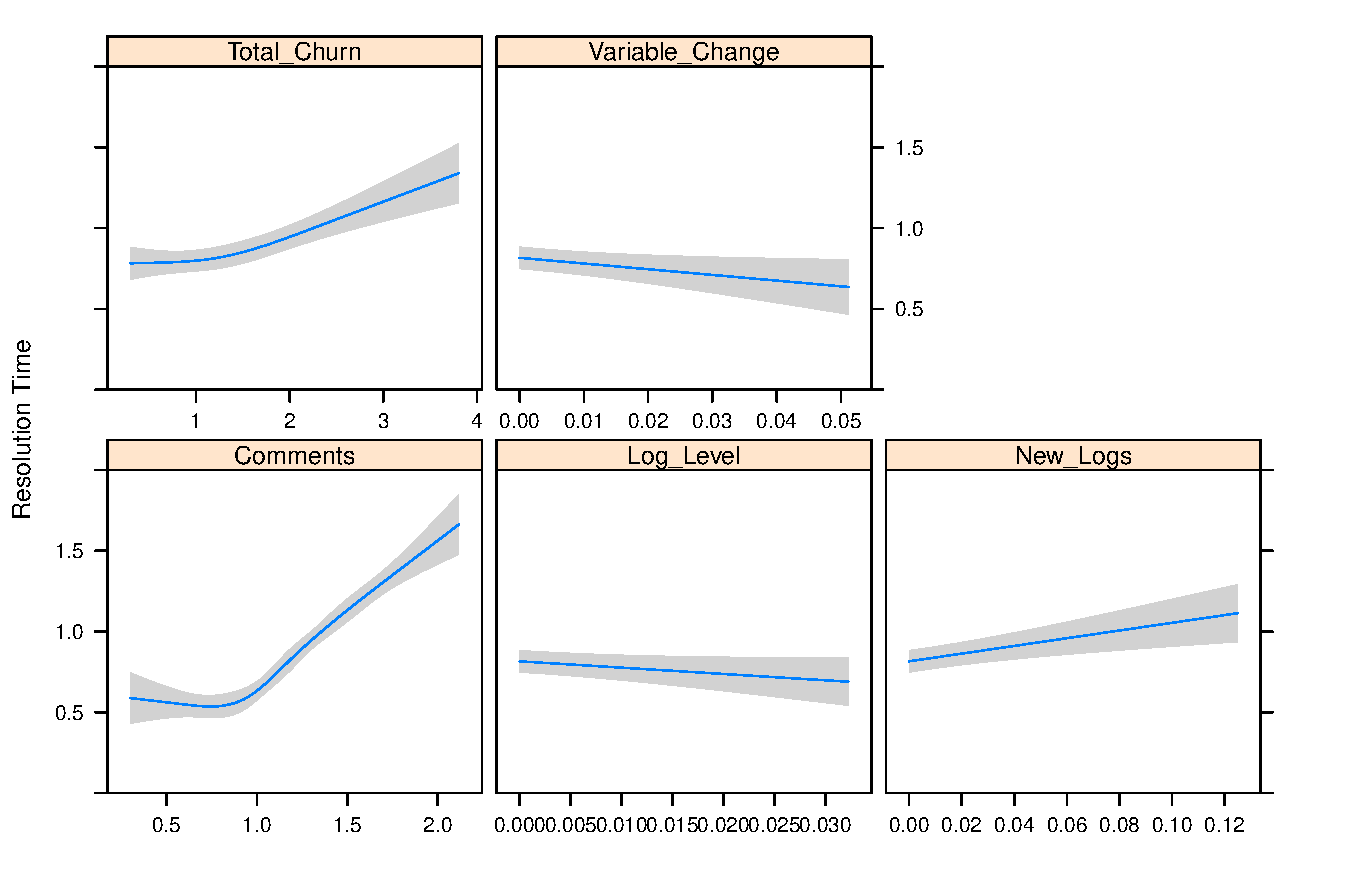
\includegraphics[width=1.45\textwidth]{HbaseDirectionPlot}
  \captionsetup[subfigure]{oneside,margin={3.5cm,-2.5cm}}

	\subcaption{HBase}
	\end{minipage}
	\hspace*{1.cm}\caption{Relation between the explanatory metrics and resolution time of bug fixing commits with log changes. Increasing graph shows increase in explanatory metrics increases the resolution time and decrease reduces the resolution time \label{fig:HbaseDirectionPlot}}
\end{figure*}

\textbf{(5) Examining explanatory metrics in relation to outcome}. Figure~\ref{fig:HbaseDirectionPlot} shows the direction of impact of log churn metrics on the resolution of bug fixes with log churn in \emph{HBase}. We find that log modifications have a negative impact on the resolution time of bug fixes. Shown in Figure~\ref{fig:HbaseDirectionPlot}, we find that in \emph{HBase} and \emph{Qpid}, modifications to logs, i.e, log level changes and variable changes are significant in the models and have negative correlations with the resolution time of bugs. 

\textbf{Modifications to log level have a negative relationship with bug resolution time.} 
We find that modifications to log level have statistically significant explanation power to bug resolution time for \emph{Qpid} and \emph{HBase}. Even though developers often do not modify log levels during bug fixes (see RQ1), our results show that changes to log levels may help in faster resolution of bugs. Although prior research finds that developers are confused when estimating the cost and benefit of each verbosity level in a log~\cite{Characterizinglogs}, a properly chosen log level may help developers diagnose filed bugs. On the other hand, a improper log level may result in too little or too much log, which are considered undesirable for diagnosing bugs~\cite{zhao2014lprof,Fu1}. An example where developers overestimate the log verbosity level is in the issue HBASE-8359\footnote{https://issues.apache.org/jira/browse/HBASE-8359}, where the log is set to \emph{info} and causes confusion among system administrators. We find that developers change the log verbosity level from \emph{info} to \emph{trace}, to reduce bulk logs being generated. On the other hand in HBASE-3401\footnote{https://issues.apache.org/jira/browse/HBASE-3401}, we see that developers underestimate the verbosity level and the log is set to default \emph{debug} and has to be updated to \emph{warn} to give more priority to the logged event. 

\textbf{Modifications to logged variables have a negative relationship with bug resolution time.} 
We find that variable changes have a statistically significant explanation power in the model for \emph{HBase} with negative relationship on the resolution time of bugs. This may be because changing information in the logs may benefit developers during bug fixes. The other reason may be that developers add new functions or keywords and leverage the new information in the logs to ensure the functionality of the new code and assure the bug is fixed~\cite{Fu1}. This enables developers to resolve the issue faster. In RQ1, we find that variable changes; especially addition and modification of logged variables is higher in bug fixes than non-bug fixes. These modifications to the logged variables highlight that developers have recognized the importance of information that is printed from logs and act on improving logs in order to assist in bug fixing.


%\begin{table}[t]
%	
%	\caption{Effect of log churn metrics on resolution time of bugs. Effect is measured by adding one standard deviation to its mean value, while the other metrics are kept at their mean values.}
%	\label{tba:SignificantFactor}
%	\begin{tabular}{|>{\centering}p{.08\textwidth}>{\centering}p{.21\textwidth}|>{\centering}p{.1\textwidth}>{\centering}p{.15\textwidth}|>{\centering}p{.1\textwidth}>{\centering}p{.15\textwidth}|}
%		\hline 
%		Delta Y  & Variable & Delta Y  & Variable & Delta Y  & Variable\tabularnewline
%		\hline 
%		\textbf{Qpid} &  & \textbf{Hadoop} &  & \textbf{HBase} & \tabularnewline
%		0.0996  & \# Comments & 0.2741  & \# Comments & 0.3562  & \# Comments\tabularnewline
%		-0.0691  & Log Level Changes & 0.0258 & Total Churn & 0.1157 & Total Churn\tabularnewline
%		&  & 0.0191  & Developers & 0.0517 & New Logs \tabularnewline
%		&  &  &  & -0.0281 & Log Level Changes\tabularnewline
%		&  &  &  & -0.0367 & Variable Changes\tabularnewline
%		\hline 
%	\end{tabular}
%	\par
%\end{table}
\textbf{New logs have a positive relationship with bug resolution time.} 
We find that new logs have a statistically significant explanation power in the model for \emph{HBase} with a positive relationship on the resolution time of bug fixes. We find that logs are often added during bug fixes in order to verify the quality of the bug fixing code. From our manual analysis results of RQ2, we find that such bugs are often complex to fix, with a large amounts of code churn and long resolution time. We compare the average code churn of bug fixes with new logs and bug fixes without new log additions. We find that the average code churn of bug fixes with new logs is almost twice that of average code churn of bug fixes without new log additions. For example, in HBASE-7305\footnote{https://issues.apache.org/jira/browse/HBASE-7305}, developers implement a read write lock for table operations to fix a race condition. This issue has total code churn over 2.5 K with over 70 new logs in the code. Because of the addition of new features this issues takes over two months to be resolved with 44 discussion posts on the issue. 


\hypobox{Log churn metrics can complement the number of comments, the number of developers and total code churn in modelling the resolution time of bugs. We find that modifications to logged variables and modifications to log level have a negative relationship with resolution time of bug fixes. On the other hand, the new logs have a positive relationship with resolution time of bugs.}






\section{Related Work}
\label{sec:Related}

In this section, we present the prior research that performs log analysis on large software systems and empirical studies on logs. 


\subsection{Log Analysis}

% The purpose of this section is to highlight the research that shows
%logs are used in debugging process. This is related to our work because
%(1) we show that logs are used in all the processes of a software
%life cycle, (2) how logs are useful in the improving the quality of
%the software. 
%\ian{some names are textsl, some are not. I think just keep the name as regular font and put et al. as italic, sometimes you miss the . in et al. and you should put dollar signs before and after the .}
Prior work leverage logs for testing and detecting anomalies in large scale systems. Shang\textsl{ et al$.$}~\cite{IanContextinformation} propose an approach to leverage logs in verifying the deployment of Big Data Analytic applications. Their approach analyzes logs in order to find differences between running in a small testing environment and a large field environment. Lou \textsl{et al}$.$~\cite{JGLouMining} propose an approach to use the variable values printed in logs to detect anomalies in large systems. Based on the variable values in logs, their approach creates invariants (e.g., equations). Any new logs that violates the invariant are considered to be a sign of anomalies. Fu \textsl{et al}$ . $~\cite{QFuanomaly} built a Finite State Automaton (FSA) using unstructured logs and to detect performance bugs in distributed systems. 

\indent Xu \textsl{et al}$ . $~\cite{ConsoleLogs} link logs to logs in source code to recover the text and and the variable parts of output logs. They applied Principal Component Analysis (PCA) to detect system anomalies. Tan \textsl{et al}$ . $~\cite{TanSalsa} propose a tool named SALSA, which constructs state-machines from logs. The state-machines are further used to detect anomalies in distributed computing platforms. Jiang \textsl{et al}$ . $~\cite{Jiang:2009:UCP:1525908.1525912} study the leverage of logs in troubleshooting issues from storage systems. They find that logs assist in a faster resolution of issues in storage systems. Beschastnikh \textsl{et al}$ . $~\cite{Beschastnikh:2011:LEI:2025113.2025151} designed automated tools that infers execution models from logs. These models can be used by developers to understand the behaviours of concurrent systems. Moreover, the models also assist in verifying the correctness of the system and fixing bugs.

To assist in fixing bugs using logs, Yuan \emph{et al$.$}~\cite{Yuan:2010:SED:1736020.1736038} propose an approach to automatically infer the failure scenarios when a log is printed during a failed run of a system.


Jiang \textsl{et al$ . $}~\cite{Jiang:2008:AAA:1400155.1400158,JiangICSM2008,JiangICSM20092,Jiang:2010:ICS:1850000.1850068} proposed log analysis approaches to assist in automatically verifying results from load tests. Their log analysis approaches first automatically abstract logs into system events~\cite{Jiang:2008:AAA:1400155.1400158}. Based on the such events, they identified both functional anomalies~\cite{JiangICSM2008} and performance degradations~\cite{JiangICSM20092} in load test results. In addition, they proposed an approach that leverage logs to reduce the load test that are performed in user environment~\cite{Jiang:2010:ICS:1850000.1850068}.

The extensive prior research of log analysis motivate our paper to study how logs are leveraged during bug fixes. As a first step, we study the changes to log during bug fixes. Our findings show that logs are change more during bug fixes than other types of code changes. The changes to logs have a relationship with a faster resolution of bugs with fewer people and less discussion.



% This is similar to our work
%because, we also use source code parsing in finding the logs. But
%instead of trying to build structured logs we try to classify them
%using levenshtein distances.

% Similar work has been done to show how mining execution logs in large systems can help  detect anomalies and ensure good load tests  \textsl{Malik et al}\cite{Automatic}. This paper  \textsl{Lou et al}\cite{JGLouMining} discuss how invariants, mined from console logs can help to detect anomalies in large systems. \textsl{Fu et al}\cite{QFuanomaly} shows analysis of unstructured logs helps in detecting performance bugs in Distributed systems. Tools have also been developed to diagnose failures by mining execution logs \textsl{Tan et al}\cite{TanSalsa}. 

%Work has been done on mining execution logs in Big Data Analytic (BDA)
%applications to find difference in behavior of the system, when tests
%are run on small testing data and actual real world data \cite{IanContextinformation}.
%Similar work has been done to show how mining execution logs in large
%systems can help in detecting anomalies and ensure good load tests
%\cite{Automatic}. In the paper execution logs are mined and event
%pair are formed. By finding patterns in these event pairs dominant
%behavior of the system is identified. Any event which does not follow
%this is tagged as anomaly and can be reported to the developers. These
%papers show that logs are not used only for the purpose of debugging
%but can assist a developer in a variety of tasks. 
%
%Research has been to detect anomalies by invariant mining\cite{JGLouMining}.
%This paper focuses on constructing structured logs from console logs.
%After construction and grouping of log messages, invariants are mined.
%Any log which violates a invariant is considered to be an anomaly.
%Unstructured log analysis has shown to be useful in detecting in even
%Distributed Systems Several \cite{QFuanomaly}. In the paper a finite
%state automaton is built and trained to automatically detect performance
%bugs in the system. These papers consider print messages and other
%unstructured logs to extract information. Then they cluster or categorize
%the logging messages into groups and logs which fall into this cluster
%are treated as anomalies. Tools have also been developed to analyze
%system logs to obtain state-machine view, control and data flow models
%and other related statistics. SALSA\cite{TanSalsa} helps in deriving
%failure diagnosis techniques and visualization for different workloads
%in Hadoop project by mining execution logs. In our study, though we
%use the same system software (Hadoop),we try to understand how logs
%can be useful in debugging and not on trying to find the bug itself. 



\subsection{Empirical studies on logs}

%In this section we try and find out how developers log. Is it done
%manually or do developers use established logging libraries. From
%our work on studying logging libraries in the Apache foundation we
%know that Slf4j, Log4j and Jakarta common logging are the most used
%libraries for logging. This helps us to find the logs
%in our case studies. Additionally there are many tools which help
%developers in logging \cite{Yuan}. The authors conduct a manual analysis and find that logs help in understanding the control and data flow in bug fixes but do not contain all the information to conclusively answer why the bug occurs. The paper addresses this issue through a tool called 'Log Enhancer' to enhance existing logs by providing additional details in the logs. This was tested with earlier version
%of the software and it was observed that 95\% of logs added by the
%tool were added by developer\textquoteright s overtime. This paper
%highlighted that do not log all the details in the first deployment
%and modify the logs in later revisions. This conforms to our findings
%as well, as we found that developers modify logs during debugging
%than other software process. 

Prior research performs an empirical study on the characteristics of logs. Yuan \textsl{et al}$ . $~\cite{Characterizinglogs} studies the logging characteristics in four open source systems. They find that over 33\% of all log changes are after thoughts and logs are changed 1.8 times more than entire code. Fu \textsl{et al$.$}~\cite{Fu1} performed an empirical study on where developer put logs. They find that logs are used for assertion checks, return value checks, exceptions, logic-branching and observing key points. The results of the analysis were evaluated by professionals from the industry and F-score of over 95\% was achieved. 


Shang \textsl{et al$ . $}~\cite{IanGap} signify the fact that there is gap between operators and developers of software systems, especially in the leverage of logs. They performed an empirical study on the evolution both static logs and logs outputted during run time~\cite{EMSEIAN,PaperIanCIIII}. They find that logs are co-evolving with the software systems. However, logs are often modified by developers without considering the needs of operators. Furthermore, Shang\textsl{ et al$ . $}~\cite{IanIcesm} find that understanding logs is challenging. They examine user mailing lists from three large open-source projects and find that users of these systems have various issues in understanding logs outputted by the system. Shang\textsl{ et al$ . $} propose to leverage different types of development knowledge, such as issue reports, to assist in understanding logs. 

Prior research by Yuan\textsl{ et al$ . $}~\cite{Yuan} shows that logs need to be improved by providing additional information. Their tool named \emph{Log Enhancer} can automatically provide additional control and data flow parameters in the logs thereby improving the output logs. Log Advisor is another tool by Zhu \emph{et al$.$}~\cite{zhu2015learning} which helps in logging by learning where developers log through existing logging instances. 

The most related prior research by Shang \emph{et al$.$}~\cite{EMSEIAN} empirically study the relationship of logging practice and code quality. Their manual analysis sheds light on the fact that some logs are changed due to field debugging. They also show that there is a strong relationship between logging practice and code quality. Our paper focused on understanding how logs are changed during bug fixes. Our results show that logs are leveraged extensively during bug fixes and may assist in the resolution of bugs. 





\section{Limitations and Threats to Validity}
\label{sec:Limit}

In this section, we discuss the threats to the validity to our findings.

\subsection*{External Validity}


Our case study is performed \emph{Hadoop}, \emph{HBase} and \emph{Qpid}. Even though these three studied projects have years of history and large user bases, the three studied projects are all Java based platform software. Systems in other domain may not rely on logs in bug fixes. More case studies on other software in other domains with other programming languages are needed to see whether our findings can be generalized. 


%The other limitation is projects in which logging data is less. We
%ran experiments on several other projects like Cassandra, Cayene,
%Zookeeper and Lucene. In all these projects the total number of logging
%statements were less to draw any meaningful conclusions. When we manually
%examined the data for Cassandra and Lucene we observed many custom
%logs which were not caught from pattern matching. As
%stated above its almost impossible to catch all instances of these
%custom logs in projects.


\subsection*{Internal Validity}


Our study is based on the data obtained from git and JIRA for all the studied systems. The quality of the data contained in the repositories can impact the internal validity of our study.

Our analysis of the relationship between changes to logs and bug resolution time cannot claim causal effects, as we are investigating correlations, rather than conducting impact studies. The explanative power of log churn metrics on the resolution time of bugs does not indicate that logs cause faster resolution of bugs. Instead, it indicates the possibility of a relation that should be studied in depth through user studies.


\subsection*{Construct Validity}

The heuristics to extract logging source code may not be able to extract every log in the source code. Even though the studied projects leverage logging libraries to generate logs at runtime, there still exist user-defined logs. By manually examining the source code, we believe that we extract most of the logs. %Evaluation on the coverage of our extracted logs can address this threat.

%We use keywords to identify bug fixes when the JIRA issue ID is not included in the commit messages.\ian{I thought you remove the commits without jira id!} Although such keywords are used extensively in prior research~\cite{EMSEIAN}, we may still miss identify bug fixes or branching and merging commits. 

We use Levenshtein ratio and choose a threshold to identify modifications to logs. However, such threshold may not accurately identify  modifications to logs. Further sensitivity analysis on such threshold is needed to better understand the impact of the threshold to our findings.

We build non-liner regression models using log churn metrics, to model the resolution time of bugs. However, the resolution time of bugs can be correlated to many factors other than just logs, such as the complexity of code fixes. To reduce such a possibility, we normalize the log churn metrics by code churn. However, other factors may also have an impact on the resolution time of bugs. Furthermore, as this is the first exploration (to our best knowledge) in modeling resolution time of bugs using log churn metrics, we are only interested in understanding the correlation between the two. Future studies should build more complex models, that consider other factors to study if there is any causation. 

Source code from different components of a system may have various characteristics. The importance of logs in bug fixes may vary in different components of the studied projects. More empirical studies on the use of logs in fixing bugs for different components of the systems are needed.



%

%commits which has type Branching in them and removed these
%branching commits from our data set. But we later found some of the
%commits are tagged under the category of UNKNOWN. When its under 'Unknown'
%category it was impossible to know if its branching or not. 

\section{Conclusion and Future Work}
\label{sec:Conclusion}
Logs are used by developers for fixing bugs. This paper is a first attempt (to our best knowledge) to understand whether logs are changed more during bug fixes and how these changes occur. The highlights of our findings are:

\begin{itemize}
	\item We find that logs are more likely to be changed during bug fixes than non-bug fixes. In particular, we find that logs are modified more likely during bug fixes than non-bug fixes. Variables and textual information in the logs are more likely to be modified during bug fixes than non-bug fixes. 
	\item We find that logs are more likely to be changed during fixing more complex bug fixes. However, bug fixes that change logs are fixed faster, need fewer developers and have less discussion.
	\item We find that log churn metrics can complement the traditional metrics such as the number of comments and the number of developers in modeling the resolution time of bugs. 
\end{itemize} 

Our findings show that logs are changed more in bug fixes and there is a relationship between changing logs and the resolution time of bugs. Developers should allocate more effort for considering the text, the logged variables and the verbosity levels in the logs the logs are added into the source code. Hence, bugs can be fixed faster without the necessity to change logs during the fix of bugs. 


% An example of a floating figure using the graphicx package.
% Note that \label must occur AFTER (or within) \caption.
% For figures, \caption should occur after the \includegraphics.
% Note that IEEEtran v1.7 and later has special internal code that
% is designed to preserve the operation of \label within \caption
% even when the captionsoff option is in effect. However, because
% of issues like this, it may be the safest practice to put all your
% \label just after \caption rather than within \caption{}.
%
% Reminder: the "draftcls" or "draftclsnofoot", not "draft", class
% option should be used if it is desired that the figures are to be
% displayed while in draft mode.
%
%\begin{figure}[!t]
%\centering
%\includegraphics[width=2.5in]{myfigure}
% where an .eps filename suffix will be assumed under latex, 
% and a .pdf suffix will be assumed for pdflatex; or what has been declared
% via \DeclareGraphicsExtensions.
%\caption{Simulation results for the network.}
%\label{fig_sim}
%\end{figure}

% Note that IEEE typically puts floats only at the top, even when this
% results in a large percentage of a column being occupied by floats.


% An example of a double column floating figure using two subfigures.
% (The subfig.sty package must be loaded for this to work.)
% The subfigure \label commands are set within each subfloat command,
% and the \label for the overall figure must come after \caption.
% \hfil is used as a separator to get equal spacing.
% Watch out that the combined width of all the subfigures on a 
% line do not exceed the text width or a line break will occur.
%
%\begin{figure*}[!t]
%\centering
%\subfloat[Case I]{\includegraphics[width=2.5in]{box}%
%\label{fig_first_case}}
%\hfil
%\subfloat[Case II]{\includegraphics[width=2.5in]{box}%
%\label{fig_second_case}}
%\caption{Simulation results for the network.}
%\label{fig_sim}
%\end{figure*}
%
% Note that often IEEE papers with subfigures do not employ subfigure
% captions (using the optional argument to \subfloat[]), but instead will
% reference/describe all of them (a), (b), etc., within the main caption.
% Be aware that for subfig.sty to generate the (a), (b), etc., subfigure
% labels, the optional argument to \subfloat must be present. If a
% subcaption is not desired, just leave its contents blank,
% e.g., \subfloat[].


% An example of a floating table. Note that, for IEEE style tables, the
% \caption command should come BEFORE the table and, given that table
% captions serve much like titles, are usually capitalized except for words
% such as a, an, and, as, at, but, by, for, in, nor, of, on, or, the, to
% and up, which are usually not capitalized unless they are the first or
% last word of the caption. Table text will default to \footnotesize as
% IEEE normally uses this smaller font for tables.
% The \label must come after \caption as always.
%
%\begin{table}[!t]
%% increase table row spacing, adjust to taste
%\renewcommand{\arraystretch}{1.3}
% if using array.sty, it might be a good idea to tweak the value of
% \extrarowheight as needed to properly center the text within the cells
%\caption{An Example of a Table}
%\label{table_example}
%\centering
%% Some packages, such as MDW tools, offer better commands for making tables
%% than the plain LaTeX2e tabular which is used here.
%\begin{tabular}{|c||c|}
%\hline
%One & Two\\
%\hline
%Three & Four\\
%\hline
%\end{tabular}
%\end{table}


% Note that the IEEE does not put floats in the very first column
% - or typically anywhere on the first page for that matter. Also,
% in-text middle ("here") positioning is typically not used, but it
% is allowed and encouraged for Computer Society conferences (but
% not Computer Society journals). Most IEEE journals/conferences use
% top floats exclusively. 
% Note that, LaTeX2e, unlike IEEE journals/conferences, places
% footnotes above bottom floats. This can be corrected via the
% \fnbelowfloat command of the stfloats package.





% conference papers do not normally have an appendix





% trigger a \newpage just before the given reference
% number - used to balance the columns on the last page
% adjust value as needed - may need to be readjusted if
% the document is modified later
%\IEEEtriggeratref{8}
% The "triggered" command can be changed if desired:
%\IEEEtriggercmd{\enlargethispage{-5in}}

% references section

% can use a bibliography generated by BibTeX as a .bbl file
% BibTeX documentation can be easily obtained at:
% http://www.ctan.org/tex-archive/biblio/bibtex/contrib/doc/
% The IEEEtran BibTeX style support page is at:
% http://www.michaelshell.org/tex/ieeetran/bibtex/
%\bibliographystyle{IEEEtran}
% argument is your BibTeX string definitions and bibliography database(s)
%\bibliography{IEEEabrv,../bib/paper}
%
% <OR> manually copy in the resultant .bbl file
% set second argument of \begin to the number of references
% (used to reserve space for the reference number labels box)


\bibliographystyle{IEEEtran}
\bibliography{Logreference}








% that's all folks
\end{document}


